\documentclass[a4paper,11pt]{book}
%\documentclass[a4paper,twoside,11pt,titlepage]{book}
\usepackage{listings}
\usepackage[utf8]{inputenc}
\usepackage[spanish]{babel}

% \usepackage[style=list, number=none]{glossary} %
%\usepackage{titlesec}
%\usepackage{pailatino}

\decimalpoint
\usepackage{dcolumn}
\newcolumntype{.}{D{.}{\esperiod}{-1}}
\makeatletter
\addto\shorthandsspanish{\let\esperiod\es@period@code}
\makeatother


%\usepackage[chapter]{algorithm}
\RequirePackage{verbatim}
%\RequirePackage[Glenn]{fncychap}
\usepackage{fancyhdr}
\usepackage{graphicx}
\usepackage{afterpage}

\usepackage{longtable}

\usepackage[pdfborder={000}]{hyperref} %referencia

% ********************************************************************
% Re-usable information
% ********************************************************************
\newcommand{\myTitle}{Diagnóstico de tumores cerebrales a partir de MRI mediante aprendizaje profundo \xspace}
\newcommand{\mySubTitle}{Diagnóstico de tumores cerebrales a partir de imágenes de resonancia magnética mediante aprendizaje profundo \xspace}
\newcommand{\myTitleENGLISH}{Brain tumor diagnosis from MRI images using deep learning \xspace}
\newcommand{\mySubTitleENGLISH}{Brain tumor diagnosis from MRI images using deep learning \xspace}
\newcommand{\myDegree}{Grado en Ingeniería Informática \xspace}
\newcommand{\myName}{Jaime Castillo Uclés\xspace}
\newcommand{\myProf}{Rosa María Rodríguez Sánchez\xspace}
%\newcommand{\mySupervisor}{Put name here\xspace}
\newcommand{\myFaculty}{Escuela Técnica Superior de Ingenierías Informática y de
Telecomunicación\xspace}
\newcommand{\myFacultyShort}{E.T.S. de Ingenierías Informática y de
Telecomunicación\xspace}
\newcommand{\myDepartment}{Ciencias de la Computación e Inteligencia Artificial \xspace}
\newcommand{\myUni}{\protect{Universidad de Granada}\xspace}
\newcommand{\myLocation}{Granada\xspace}
\newcommand{\myTime}{\today\xspace}
\newcommand{\myVersion}{Version 0.1\xspace}


\hypersetup{
pdfauthor = {\myName jaimecastillo@correo.ugr.es},
pdftitle = {\myTitle},
pdfsubject = {},
pdfkeywords = {palabra_clave1, palabra_clave2, palabra_clave3, ...},
pdfcreator = {LaTeX con el paquete ....},
pdfproducer = {pdflatex}
}

%\hyphenation{}


%\usepackage{doxygen/doxygen}
\usepackage{pdfpages}
\usepackage{url}
\usepackage{colortbl,longtable}
\usepackage[stable]{footmisc}
%\usepackage{index}

%\makeindex
%\usepackage[style=long, cols=2,border=plain,toc=true,number=none]{glossary}
% \makeglossary

% Definición de comandos que me son tiles:
%\renewcommand{\indexname}{Índice alfabético}
%\renewcommand{\glossaryname}{Glosario}

\pagestyle{fancy}
\fancyhf{}
\fancyhead[LO]{\leftmark}
\fancyhead[RE]{\rightmark}
\fancyhead[RO,LE]{\textbf{\thepage}}
\renewcommand{\chaptermark}[1]{\markboth{\textbf{#1}}{}}
\renewcommand{\sectionmark}[1]{\markright{\textbf{\thesection. #1}}}

\setlength{\headheight}{1.5\headheight}

\newcommand{\HRule}{\rule{\linewidth}{0.5mm}}
%Definimos los tipos teorema, ejemplo y definición podremos usar estos tipos
%simplemente poniendo \begin{teorema} \end{teorema} ...
\newtheorem{teorema}{Teorema}[chapter]
\newtheorem{ejemplo}{Ejemplo}[chapter]
\newtheorem{definicion}{Definición}[chapter]

\definecolor{gray97}{gray}{.97}
\definecolor{gray75}{gray}{.75}
\definecolor{gray45}{gray}{.45}
\definecolor{gray30}{gray}{.94}

\lstset{ frame=Ltb,
     framerule=0.5pt,
     aboveskip=0.5cm,
     framextopmargin=3pt,
     framexbottommargin=3pt,
     framexleftmargin=0.1cm,
     framesep=0pt,
     rulesep=.4pt,
     backgroundcolor=\color{gray97},
     rulesepcolor=\color{black},
     %
     stringstyle=\ttfamily,
     showstringspaces = false,
     basicstyle=\scriptsize\ttfamily,
     commentstyle=\color{gray45},
     keywordstyle=\bfseries,
     %
     numbers=left,
     numbersep=6pt,
     numberstyle=\tiny,
     numberfirstline = false,
     breaklines=true,
   }
 
% minimizar fragmentado de listados
\lstnewenvironment{listing}[1][]
   {\lstset{#1}\pagebreak[0]}{\pagebreak[0]}

\lstdefinestyle{CodigoC}
   {
	basicstyle=\scriptsize,
	frame=single,
	language=C,
	numbers=left
   }
\lstdefinestyle{CodigoC++}
   {
	basicstyle=\small,
	frame=single,
	backgroundcolor=\color{gray30},
	language=C++,
	numbers=left
   }

 
\lstdefinestyle{Consola}
   {basicstyle=\scriptsize\bf\ttfamily,
    backgroundcolor=\color{gray30},
    frame=single,
    numbers=none
   }


\newcommand{\bigrule}{\titlerule[0.5mm]}


%Para conseguir que en las páginas en blanco no ponga cabecerass
\makeatletter
\def\clearpage{%
  \ifvmode
    \ifnum \@dbltopnum =\m@ne
      \ifdim \pagetotal <\topskip
        \hbox{}
      \fi
    \fi
  \fi
  \newpage
  \thispagestyle{empty}
  \write\m@ne{}
  \vbox{}
  \penalty -\@Mi
}
\makeatother

\begin{document}
\begin{titlepage}
 
\newlength{\centeroffset}
\setlength{\centeroffset}{-0.5\oddsidemargin}
\addtolength{\centeroffset}{0.5\evensidemargin}
\thispagestyle{empty}

\noindent\hspace*{\centeroffset}\begin{minipage}{\textwidth}

\centering

\includegraphics[width=0.9\textwidth]{imagenes/logoUGR.jpg}\\[1.4cm]

\textsc{ \Large TRABAJO FIN DE GRADO\\[0.2cm]}
\textsc{ INGENIERÍA INFORMÁTICA}\\[1cm]
% Upper part of the page

% Title
{\LARGE \bfseries \myTitle \\}
\noindent\rule[-1ex]{\textwidth}{3pt}\\[3.5ex]
{\large\bfseries \mySubTitle}
\end{minipage}

\vspace{2.5cm}
\noindent\hspace*{\centeroffset}\begin{minipage}{\textwidth}
\centering

\textbf{Autor}\\ {\myName}\\[2.5ex]
\textbf{Directora}\\
{\myProf}\\[2cm]

\includegraphics[width=0.3\textwidth]{imagenes/etsiit_logo.png}\hspace{1.0cm}

\includegraphics[width=0.1\textwidth]{imagenes/decsai_logo.png}\\[0.25cm]
\textsc{Escuela Técnica Superior de Ingenierías Informática y de Telecomunicación}\\
\textsc{---}\\
Granada, Junio de 2024
\end{minipage}
%\addtolength{\textwidth}{\centeroffset}
%\vspace{\stretch{2}}
\end{titlepage}



\chapter*{}
%\thispagestyle{empty}
%\cleardoublepage

%\thispagestyle{empty}
\cleardoublepage
\thispagestyle{empty}

\begin{center}
{\large\bfseries \myTitle: \mySubTitle}\\
\end{center}
\begin{center}
\myName\\
\end{center}

%\vspace{0.7cm}
\noindent{\textbf{Palabras clave}: palabra\_clave1, palabra\_clave2, palabra\_clave3, ......}\\

\vspace{0.7cm}
\noindent{\textbf{Resumen}}\\

Poner aquí el resumen.
\cleardoublepage

\thispagestyle{empty}

\begin{center}
{\large\bfseries \mySubTitleENGLISH: \mySubTitleENGLISH}\\
\end{center}
\begin{center}
\myName\\
\end{center}

%\vspace{0.7cm}
\noindent{\textbf{Keywords}: Keyword1, Keyword2, Keyword3, ....}\\

\vspace{0.7cm}
\noindent{\textbf{Abstract}}\\

Write here the abstract in English.

\chapter*{}
\thispagestyle{empty}


\noindent\rule[-1ex]{\textwidth}{2pt}\\[4.5ex]

Yo, \textbf{\myName}, alumno de la titulación \myDegree de la \textbf{Escuela Técnica Superior
de Ingenierías Informática y de Telecomunicación de la Universidad de Granada}, con DNI 45924736S, autorizo la
ubicación de la siguiente copia de mi Trabajo Fin de Grado en la biblioteca del centro para que pueda ser
consultada por las personas que lo deseen.

\vspace{6cm}

\noindent Fdo: \myName

\vspace{2cm}

\begin{flushright}
Granada a X de Junio de 2024 .
\end{flushright}


\chapter*{}
\thispagestyle{empty}

\noindent\rule[-1ex]{\textwidth}{2pt}\\[4.5ex]

Dña. \textbf{\myProf}, Profesor del Área de \myDepartment del Departamento de \myDepartment de la Universidad de Granada.


\vspace{0.5cm}

\textbf{Informan:}

\vspace{0.5cm}

Que el presente trabajo, titulado \textit{\textbf{\myTitle, \mySubTitle}},
ha sido realizado bajo su supervisión por \textbf{\myName}, y autorizamos la defensa de dicho trabajo ante el tribunal
que corresponda.

\vspace{0.5cm}

Y para que conste, expiden y firman el presente informe en Granada a X de mes de 2024 .

\vspace{1cm}

\textbf{La directora:}

\vspace{5cm}

\noindent \textbf{}

\chapter*{Agradecimientos}
\thispagestyle{empty}

       \vspace{1cm}


Poner aquí agradecimientos...
\frontmatter
\tableofcontents
\listoffigures
\listoftables
%
\mainmatter
%\setlength{\parskip}{5pt}
\addcontentsline{toc}{chapter}{Introducción}
\chapter{Introducción}

Los tumores cerebrales son una de las formas más letales de cáncer. Específicamente, los glioblastomas y sus variantes difusas son los más comunes y agresivos tipos de tumor del sistema nervioso central en adultos. Su alta heterogeneidad en apariencia, forma e histología los convierte en una de las patologías más difíciles de diagnosticar, de tratar y un reto para el campo de la imagen médica.

Desde el punto de vista de la ingeniería y la informática, vemos como sin duda la aplicación de técnicas de Visión por Computador es una de las máximas para la investigación en imagen médica en la actualidad. Sólo considerando su aplicación en el diagnóstico de enfermedades, desde 2008 el número de publicaciones promedio realizadas por año se ha incrementado notablemente tanto que actualmente es diez veces mayor que en sus inicios. 

Resultados notables como la inclusión de robots especializados para la cirugía \cite{DAVINCI} o buenos resultados en competiciones de ciencia de datos que replican la precisión médica \cite{PANDA} evidencian esta tendencia. El trabajo conjunto de personal médico e ingenieros promete seguir dando resultados que de forma separada eran inaccesibles.



\section{Objetivos}

**Hablar sobre porqué al dejar la tarea de segmentar a una máquina esta puede ser más precisa que un humano**

Con este trabajo se pretende perseguir la creación de una arquitectura que mejore el estado del arte actual para equipar a un programa al servicio de personal médico para la ayuda en la evaluación del diagnóstico de un posible paciente de tumor cerebral.

A continuación, detallaremos de una forma más profunda estos objetivos.

El cerebro no tiene terminaciones nerviosas. Los pacientes no sienten dolor a causa de un tumor cerebral por sí mismo. Generalmente, acaban buscando ayuda médica por la aparición de otros indicios relacionados difíciles de distinguir de otras patologías agudas y de mucho menor transcendencia (visión borrosa, pérdida del control, etc).

Los glioblastomas y sus variantes tienen una media de supervivencia de 15 meses tras su diagnóstico.

En general, los tumores cerebrales son difíciles de tratar y son resistentes a terapias convencionales usadas en otros tipos de cánceres como la quimioterapia debido a los desafíos que presenta el cerebro para tolerar ciertos químicos, transportar medicamentos dentro de él y la alta importancia que tiene en este órgano la optimización del uso de tratamientos que puedan ser invasivos. En otras palabras, el uso de tratamientos basados en la extirpación o en la medicación pueden ser arriesgados. Por tanto, el tratamiento más común de estos está basado en la radioterapia.


\section{Metodología}


\addcontentsline{toc}{chapter}{Estado del arte}
\chapter{Estado del arte}

En este capítulo estudiaremos y analizaremos los diferentes enfoques para nuestra principal tarea, \textbf{la segmentación de tumores cerebrales}. Abordando desde el inicio del estudio del problema pasando por la explosión de métodos basados en Aprendizaje profundo con la constitución de \textbf{BraTS} hasta nuestros días. Se pondrá especial énfasis a las soluciones actuales comparándolas desde sus diferencias en metodología y perspectiva.

Otras tareas contenidas en el diagnóstico completo de tumores cerebrales como la clasificación de tumores cerebrales (glioblastomas y meningiomas) o la predicción de su evolución, que se recogen en este trabajo, van intrínsecamente unidas al buen desempeño de la tarea de segmentación. 

Por un lado, la clasificación entre los dos tipos de tumores no es tan relevante a la hora de diseñar un sistema de ayuda a la toma de decisión ya que clínicamente sí existe una característica diferencial entre ambos, su \textbf{localización}. Los meningiomas siempre aparecen entre el cráneo y el cerebro no internamente en el cerebro como los glioblastomas. Esto hace que un médico pueda distinguirlos sin requerir una gran asistencia de una máquina para la mayoría de los casos. Adicionalmente, la clasificación de por sí ayuda a la toma de decisiones en el tratamiento pero no es el elemento crítico para la supervivencia del paciente que depende de la eliminación del tumor donde su segmentación toma un papel crucial.

Por otro lado, la tarea de la predicción de la evolución del tumor se representa como la predicción de la segmentación en un estado futuro del tumor es decir depende fuertemente de la segmentación actual del tumor. 

Es por ello que grandes esfuerzos se han realizado en entorno a la segmentación, ya que otras tareas que conforman su diagnóstico se verían arrastradas.

Diferentes dificultades han sido las que a pesar de años de desarrollo aún encontrar un algoritmo para la segmentación de tumores cerebrales sea algo mejorable. 

\begin{enumerate}
	\item \textbf{Incertidumbre en la localización} : Como vimos no existe una zona concreta en general para la aparición de los tumores cerebrales. A excepción, de los meningiomas localizados en zonas superficiales del cerebro y aún siendo una región muy amplia, incluso ya desarrollado un tumor pueden aparecer otros localizados en regiones muy distintas de la original. 
	\item \textbf{Incertidumbre en la morfología} : A diferencia de otras patologías, cada tumor cerebral presenta un tamaño y forma completamente distintas y donde en principio no se puede apreciar un patrón distintivo. Esto hace que sea muy complicado y generalmente aporte malos resultados, la construcción de sistemas basados reglas u otras aproximaciones que no incluyen una componente de aprendizaje.
	
	\item \textbf{Bajo contraste} : Una buena resolución y contraste son características muy importantes para entender la información de una imagen. Las imágenes IRM producidas en una resonancia debido a proyecciones de imagen y procesos de tomografía usualmente ofrecen una baja resolución y contraste haciendo más difícil la definición de bordes entre diferentes tejidos de la imagen. Una segmentación precisa es difícil de conseguir.
	
	\item \textbf{Sesgo en las etiquetas}. Existen indicios para pensar que las etiquetas proporcionadas pueden presentar ruido. El proceso de segmentado por parte del personal médico 
	depende de su experiencia profesional lo cual puede llevar a cometer errores. Por ejemplo, se han presentado eventualmente discrepancias entre distintos anotadores: algunos tienden a conectar todas las pequeñas regiones de un tejido mientras que otros las segmentan de forma más precisa y separada. 
	
	\item \textbf{Desbalanceo en el tejido} : Dentro de la segmentación entre los diferentes tipos de tejidos, usualmente existe un tejido NCR que es usualmente más pequeño que los otros dos. 
	Esto podría afectar en el proceso de aprendizaje hacia una pobre generalización de este tipo de tejido. 
	
	\item \textbf{Desbalanceo entre pacientes} : En el conjunto de datos tenemos muchos pacientes de norteamerica y de ascendencia blanca, pero pocos de otros origenes como el africano. Además, de tener un sesgo claro de edad ya que existen pocos casos en niños. Esta falta de datos puede impedir que exista una buena generalización para estos casos más aislados.
	
\end{enumerate}



\section{Revisión histórica}

	A continuación, se presenta una revisión histórica sobre la segmentación de tumores cerebrales hasta 2021 apoyada en \cite{liu2023deep}. Se presenta una línea del tiempo con los principales trabajos de estudio.
	
	\begin{figure}[!h]
		\centering
		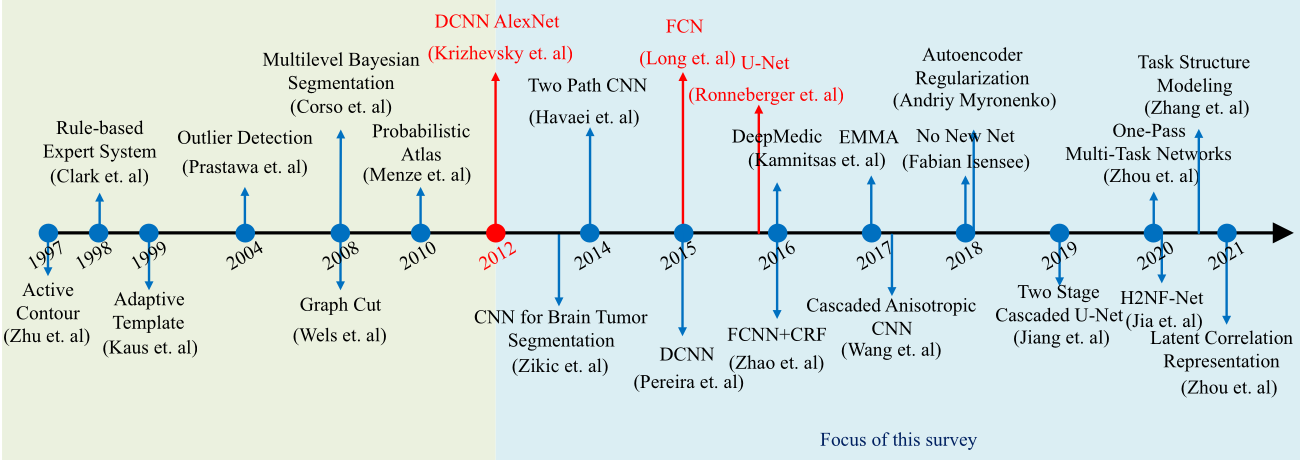
\includegraphics[width=1.0\linewidth]{imagenes/evolution_stateofart.png}
		\caption{Evolución histórica del estado del arte hasta 2021.}
	\end{figure}
	
	En la década de 1990 investigadores como \cite{zhu1997computerized} fueron pioneros al utilizar una red Hopfield con un modelo de contornos activos para extraer los bordes del tumor. Sin embargo, incluso el entrenamiento de una pequeña red como esta era algo computacionalmente costoso por las limitaciones de la época.  Desde 1990 hasta 2012, los métodos que iban surgiendo para la segmentación de tumores cerebrales estaban basados en métodos clásicos de aprendizaje con características extraídas a mano, sistemas expertos que se apoyaban en los histogramas de la imagen, plantillas para la segmentación y modelos gráficos. 
	
	A pesar de ser un gran paso inicial, tenían grandes deficiencias. Por ejemplo, la mayoría de ellos sólo se centraba en la segmentación de todo el tumor lo cual lleva a un modelo poco útil. Por otro lado, en los modelos basados en características extraídas se hacía muy tedioso poder usarlos eficazmente ya que este paso de extracción dependía de conocimiento previo experto que en ningún momento se pudo llegar a representar en un modelo. En último lugar, los mismos problemas que compartimos hoy en día sobre el desbalanceo y la incertidumbre del problema eran mucho más agresivos. 
	
	Tras 2012 con la revolución del Deep Learning, se introducen nuevas tecnologías (Redes neuronales convolucionales y U-net) que mejorarán los resultados obtenidos hasta el momento. 
	Se empezarán a construir arquitecturas encoder-decorder convolucionales para conseguir pipelines completos para la segmentación. El aprendizaje profundo toma el problema de lleno proclamándose el enfoque que define el estado del arte.
	
	Podemos clasificar las soluciones basadas en aprendizaje profundo aportadas en tres categorías según el principal problema para que el están pesadas. Sin embargo, como veremos en las soluciones más actuales lo ideal es tratar con los tres problemas.
	
	\subsection{Métodos que se enfocan en la arquitectura}
		
		 Para poder obtener redes que automáticamente extraen características discriminativas a altas dimensiones es necesario un efectivo diseño de módulos y arquitecturas. Por un lado, se pretende que la arquitectura sea capaz de aprender semánticamente y a localizar regiones de interés por medio de añadir profundidad a la red, a través de mecanismos de atención o la fusión de características entre las resonancias. Por otro lado, se pretende minimizar la cantidad de parámetros entrenables de la red o conseguir un entrenamiento más rápido.
		 
		\subsubsection{Diseño de bloques especializados}
			
			Los primeros trabajos que tenían este objetivo comenzaron por basarse en arquitecturas bien conocidas como AlexNet o VGGNet a través del uso de una secuencia de imágenes de la resonancia completa como entrada.
			
			Para la mejora de resultados, se optó por introducir todas las resonancias como entrada de la red y añadir más capas convolucionales. Con ello, teníamos redes más profundas pero que pronto empezaban a sufrir los problemas del explosión y desvanecimiento del gradiente durante el proceso de entrenamiento. Para ayudar a lidiar con estos problemas, se introdujo a las redes, \textbf{conexiones residuales}.
			Conectando la entrada de la red con su salida, convergiendo más rápido y con mejores resultados. 
			
			Este proceso de aumento de profundidad con conexiones residuales no sería definitivo porque también conlleva el sacrificio de resolución espacial. Se reemplazaría en trabajos siguientes, el uso de la convolución simple por convoluciones dilatadas. El \textbf{uso de convoluciones dilatadas} traería el aumento del espacio receptivo (ya que se aplica una convolución a un espacio mayor de la imagen) sin necesidad de introducir parámetros a la red. La convolución dilatada se vería especialmente útil por ejemplo en la segmentación de áreas grandes como suele ocupar el tejido ED (edema tumoral). 
			
			Respecto conseguir una buena eficiencia en tiempo de entrenamiento es conocido aplicar un reordenamiento en memoria de las imágenes de la resonancia similares (p. ej. el mismo slice en las 4 pruebas) de forma que reduzcan la comunicación entrada-salida con GPU. Adicionalmente, se utilizan \textbf{conexiones reversibles} en la red de forma que durante el proceso de backpropagation (backward pass) no se necesite memoria adicional para guardar las activaciones intermedias y la aplicación de la combinación \textbf{convoluciones separables} para cada convolución standard necesaria por motivos de eficiencia. 
			
			\begin{figure}[!h]
				\centering
				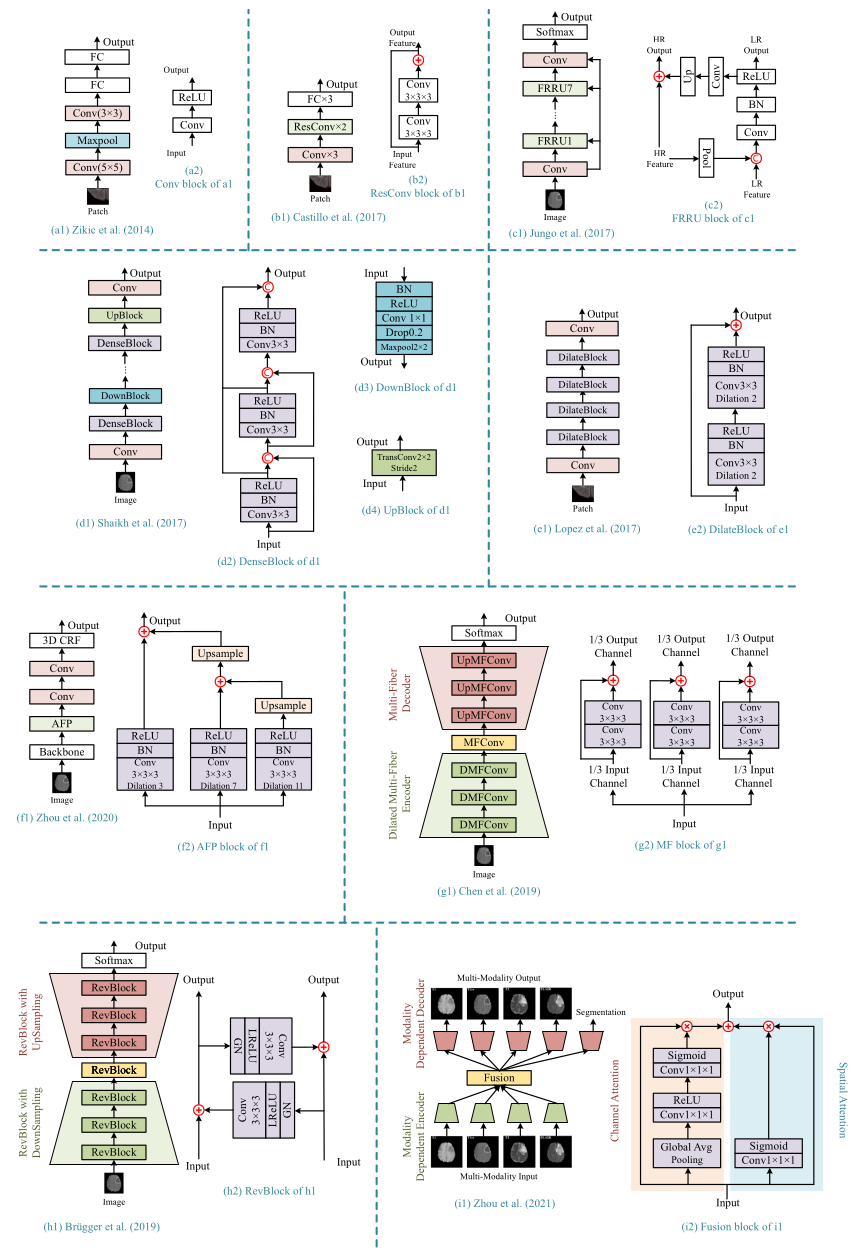
\includegraphics[width=1.0\linewidth]{imagenes/estructura_revisionhistorica.png}
				\caption{Estructura de las arquitecturas de esta revisión.}
			\end{figure}
			
			\subsubsection{Diseño de arquitecturas efectivas}
			
			La mayoría de los trabajos de recorrido histórico se encasillan en alguno de los siguientes dos enfoques de arquitectura: \textbf{redes neuronales convolucionales} para extraer características de la imagen y clasificar los píxeles de la imagen según las etiquetas de los tejidos posibles o \textbf{redes encoder-decoder} en las cuales se puede definir un pipeline completo convolucional sin la necesidad de la agregación de capas totalmente conectadas.
			
			\begin{enumerate}
					
				\item \textbf{Redes neuronales convolucionales de una/múltiples trayectorias}
					
					
				A diferencia de una red convolucional de una única trayectoria, las redes de trayectoria múltiples tienen la capacidad de extraer diversas características a diferentes escalas. Estas características se combinan para su posterior procesamiento, permitiendo a las redes aprender tanto características globales como locales. 
				
				\begin{figure}[!h]
					\centering
					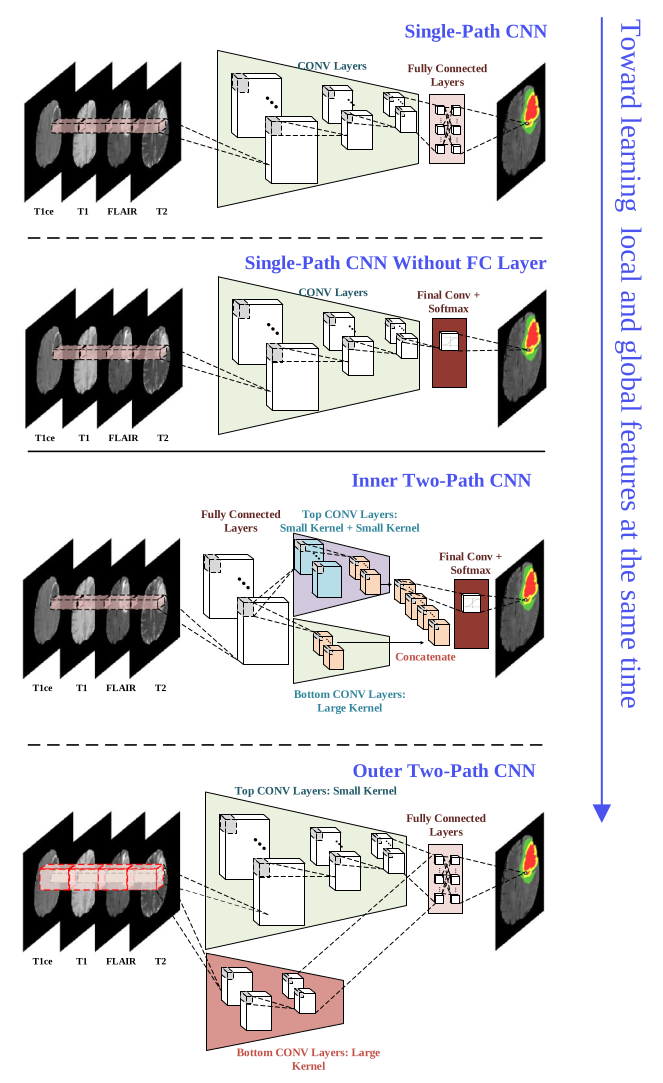
\includegraphics[width=0.5\linewidth]{imagenes/comparisonsinglemultipleCNN.png}
					\caption{Comparación entre arquitecturas de una y múltiples trayectorias. Imagen de \cite{liu2023deep}}
				\end{figure}
				
				Por ejemplo, \cite{havaei2017brain} desarrollaron una estructura de dos vías que integra información tanto local como global del tumor, utilizando núcleos de convolución de diferentes tamaños.
				
				\begin{figure}[!h]
					\centering
					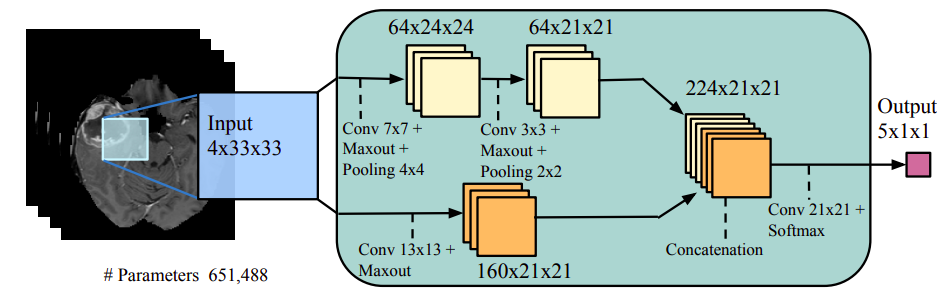
\includegraphics[width=0.75\linewidth]{imagenes/havaei2017architecture.png}
					\caption{Arquitectura de dos vías de \cite{havaei2017brain}}
				\end{figure}
				
				Otros enfoques, como el de \cite{kamnitsas2017efficient}, optan por aprender información global localmente desde la entrada misma, utilizando redes de doble vía patches de diferentes tamaños y pequeños núcleos de convolución. 
				
				Este tipo de arquitecturas fueron una de las primeras aproximaciones que empezaban adaptarse con éxito a las complejidades de la segmentación de tumores cerebrales.
				
					
				\item \textbf{Arquitecturas Encoder-Decoder}
					
			\end{enumerate}
			
			
		\subsection{Métodos que tratan el desbalanceo}
			\subsubsection{Métodos multi-red}
			\begin{enumerate}
					
				\item \textbf{Redes en cascada}
					
				\item \textbf{Ensamblado de modelos}
					
			\end{enumerate}
				
			\subsubsection{Funciones de pérdida especializadas}
		
		
		\subsection{Métodos que tratan la información multi-modal}


\section{Enfoques actuales}
	\subsection{Basados en CNN}
	
	Como vimos anteriormente históricamente existen referencias muy buenas de forma independiente por tratar de conseguir una arquitectura efectiva, evitar los problemas asociados al desbalanceo y sacarle partido a la información multi-modal. En aproximaciones más reciente se intenta unificar estos propósitos con el fin de un desempeño mayor en el problema.
	
	
	
	
	\subsection{Basados en Transformers}



\addcontentsline{toc}{chapter}{Metodología}
\chapter{Metodología}

En este capítulo describimos en profundidad todos los pasos seguidos en los métodos empleados en el trabajo y su justificación. Posteriormente, se aplicarán en la experimentación.

\section{Análisis de los recursos disponibles}

Para la realización de este trabajo debemos considerar los recursos hardware disponibles para la inferencia de los modelos pero sobre todo para el entrenamiento de los modelos.

\begin{enumerate}
	\item \textbf{Hardware en entrenamiento}. Para el desarrollo de toda la experimentación, entrenamiento de los modelos y validación nos valdremos de los recursos que gratuitamente ofrece Kaggle, una plataforma de ciencia de datos propiedad de Google. 
	
	El recurso más importante que ofrece Kaggle y razón de su uso es que nos permite el uso de su gráfica NVIDIA Tesla P100 por 30 horas semanales. Con ella, podemos entrenar los modelos y hacer una inferencia rápida para validación en tiempo razonable.
	
	Los recursos locales que dispongo son un ordenador personal que aunque con mejor capacidad de memoria en disco $\approx 2\ TB$ que la ofrecida por Kaggle $\approx 100\ GB$, nuestra gráfica NVIDIA GeForce RTX 2060 tiene inmensamente menores prestaciones que la ofrecida en Kaggle. A continuación, mostramos una gráfica de rendimiento sobre las características de ambos dispositivos para cuantificar este hecho.
	
	\begin{figure}[H]
		\centering
		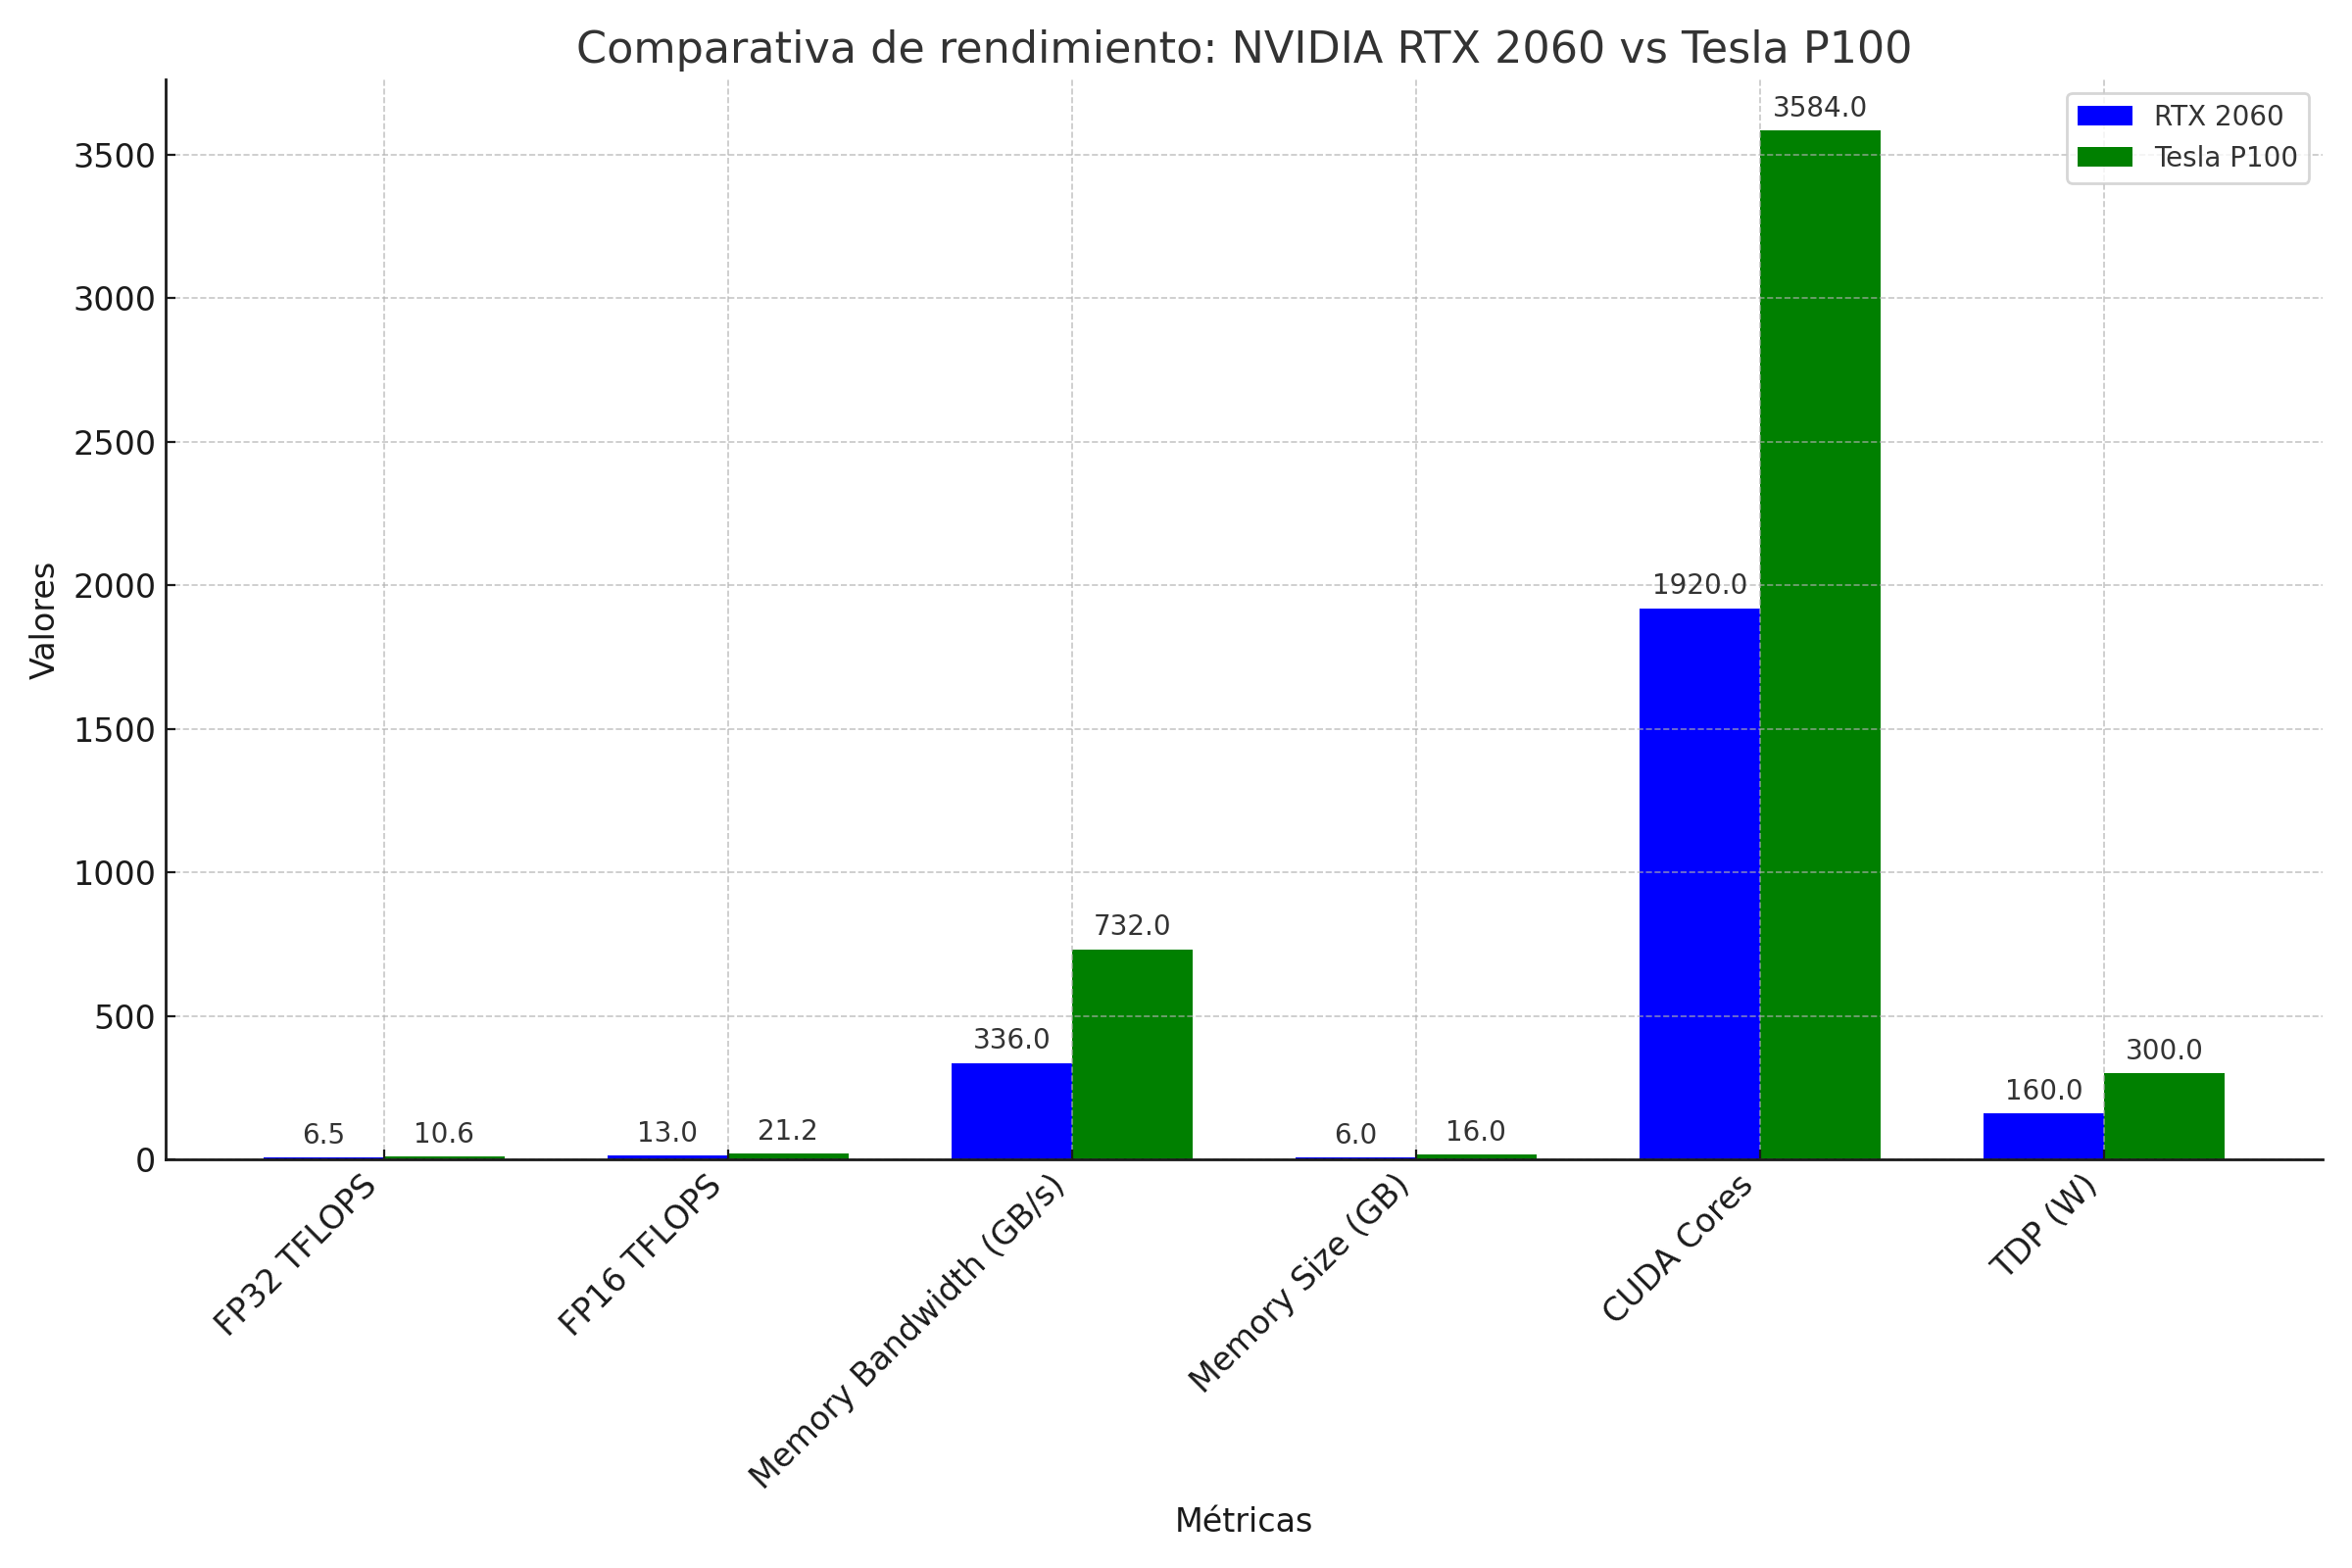
\includegraphics[width=1.0\linewidth]{imagenes/comparativa_rtx2060tesla.png}
		\caption{Comparativa de rendimiento de las GPU disponibles}
	\end{figure}
	
	En todas las características la gráfica ofrecida por Kaggle supera a la nuestra. Por lo que optaremos por usarla en todo el trabajo.
	
	\item \textbf{Hardware para inferir con los modelos}. Para la construcción de la interfaz y su uso si hemos usado nuestro dispositivo personal.
	
	De forma general, el hardware necesario para inferir con los modelos es cualquier PC de uso personal que disponga de una GPU de rendimiento similar o mejor que el nuestro y cumpla las siguientes dependencias (link a apéndice de uso del programa). 
	
\end{enumerate}


\section{Preprocesado de Datos}

En este apartado se explicará el preprocesamiento que se ha aplicado a las resonancias magnéticas para convertirlas a entradas de los modelos. 

Partiendo de nuestro conjunto de datos que presentamos en la introducción obtenido de la competición \textbf{BraTS} en Synapse. Ya vemos como las resonancias presentan características favorables para ser una entrada a la red.

\begin{enumerate}
	\item \textbf{Dimensiones estandarizadas} : Todas las resonancias (adultos, niños, diferente tipo de tumor) presentan las mismas dimensiones.
	\item \textbf{Imágenes estandarizadas} : Todas las resonancias se han hecho con el mismo estándar de escáner, todas presentan el mismo rango para su visualización. 
	\item \textbf{No existen valores faltantes} : Observamos como el conjunto de datos es completo en su definición, todas las resonancias de cada paciente tienen las mismas cuatro pruebas.
\end{enumerate}

\subsection{Elección de dimensionalidad de las entradas}

Una de las elecciones cruciales al inicio del trabajo es la dimensionalidad de las entradas de la red (determina la forma en la que se procesan los datos). ¿Es mejor trabajar en 2D con una única imagen como entrada o en 3D con todo el conjunto de imágenes de una resonancia como entrada?

En un primer momento debido a que la mayoría de literatura actual trabaja en 3D, intentamos trabajar en 3D. Para ello, construimos un primer modelo inicial de arquitectura para 2D y  una forma de transformarlo a 3D es simplemente duplicar cada capa por la cantidad de imágenes en cada resonancia. Por lo que, el tamaño de nuestro modelo inicial 2D $SIZE_{2D}$ sólo debíamos multiplicarlo por la cantidad de imágenes en una resonancia $SIZE_{3D} = SIZE_{2D} \times 155 $. Debido que el máximo de memoria RAM que disponíamos en la Tesla P100 de Kaggle es $16\ GB$ siguiendo esa regla, el máximo tamaño que podría ocupar un modelo inicial 2D sería: 

$$ MAXSIZE_{2D} = \frac{16\ GB}{155}  = 0.10323\ GB = 105.7\ MB $$  

Esta cantidad de memoria para una arquitectura que obtenga resultados competentes en la actualidad de técnicas que existen no es viable. Viéndonos obligados ante la escasez de memoria en GPU a enfocar nuestros esfuerzos en una dimensionalidad 2D. Tendremos como entrada a las arquitecturas \textbf{una única imagen la correspondiente a la vista axial de las resonancias}.

\subsection{Normalizado de las imágenes}

Las imágenes que componen las resonancias son mapas en escala de gris donde un píxel de la imagen puede tomar un valor de gris en el intervalo $[0, 256)$. Entre las imágenes de distintas resonancias se encuentra una misma distribución de valores de píxeles para representar la misma información. Sin embargo, el proceso de entrenamiento no deja de ser un proceso de optimización y puede que este rango sea aún demasiado grande.

Adicionalmente, para evitar posibles píxeles erróneos en la toma de las imágenes que podamos interpretar como outliers que tengan un impacto negativo en el entrenamiento y para hacer las imágenes más interpretables se aplica a las imágenes normalización Z-score o estandarización.

$$ X_{std}^{i}= \frac{x^{i}-mean}{std} $$



\subsection{Recortado de imagen}

Podría ser razonable reducir las dimensiones de las imágenes para hacer que los datos sean menos pesados. Sin embargo, se opta por no hacerlo por seguridad y escalibilidad. \textbf{BraTS} fija esas dimensiones en base al estándar en una resonancia magnética, así para cualquier paciente se garantiza que la imagen de su cerebro se puede representar en una resonancia en unas condiciones de resolución iguales al resto de pacientes.

Si recortamos las imágenes de forma cuadrada al cerebro más grande de todas las resonancias, podríamos encontrarnos en inferencia con un cerebro mayor que no se podría representar en una imagen. Es necesario dejar cierto margen, optando por respetar el margen inicial que marcan los organizadores médicos de \textbf{BraTS}.

\subsection{Undersampling}

En el estado del arte ya mencionamos que existía un desbalanceo entre tejido sano y tejido enfermo. En la mayoría de resonancias existe una mayor proporción de tejido sano que de tejido enfermo. Esto no sólo podía introducir un sesgo en los algoritmos de segmentación sino que aumenta mucho el coste computacional de entrenar a los modelos por el exceso de imágenes que no contienen la información de una lesión tumoral. 

El tratamiento del desbalanceo mediante undersampling siempre es una medida agresiva ya que podría eliminar información que a priori no consideramos relevante y si lo es.

Sin embargo, en nuestro problema aplicaremos undersampling con el principal objetivo de reducir los tiempos de entrenamiento y poder tener una arquitectura más profunda manteniendo tiempos razonables. Intentando aliviar de paso el problema del desbalanceo.
A continuación explicamos en detalle como se ha llevado a cabo.

Para todo nuestro conjunto de datos $X$ creamos archivos CSV para cada partición (entrenamiento, validación y test) donde cada fila de cada archivo CSV representa a una imagen o entrada a la red. 

Estos archivos en formato CSV contendrán únicamente el conjunto de imágenes que contienen lesión tumoral de todas las resonancias $N$ más una parte seleccionada aleatoriamente de imágenes sin lesión de tamaño $\frac{|N|}{2}$. De esta forma, nos quedamos con todas las imágenes con información de lesión y con una parte representativa y balanceada sin lesión para no sesgar al modelo a segmentar en todas las imágenes.

Este es el pseudo-código de creación de los archivos CSV para este proceso de undersampling. 

\begin{algorithm}
	\caption{Undersampling de las imágenes a usar}
	\begin{algorithmic}[1]
		\STATE \textbf{Entrada:} \textit{mri\_paths}, \textit{name}
		\STATE \textbf{Salida:} Archivo CSV con columnas (t1c, t1n, t2f, t2w, slice, etiqueta)
		\STATE \textbf{Inicializar} lista vacía \textit{data}
		
		\FOR{cada \textit{mri\_path} en \textit{mri\_paths}}
		\STATE \textit{label\_path} $\gets$ \textit{mri\_path[1]}
		\STATE \textit{label\_img} $\gets$ Cargar \textit{label\_path}
		\FOR{\textit{slice\_num} en rango(5, 150)}
		\IF{hay algún tumor en \textit{label\_img[:, :, slice\_num]}}
		\STATE \textit{label} $\gets$ 0 si "MEN" $\in$ \textit{label\_path}, sino 1
		\STATE Añadir \{t1c, t1n, t2f, t2w, slice, etiqueta\} a \textit{data}
		\ENDIF
		\ENDFOR
		\STATE Liberar \textit{label\_img} y recolectar basura
		\ENDFOR
		
		\STATE \textit{notumores\_size} $\gets$ longitud de \textit{data} dividido 2
		\FOR{cada $i$ en rango(0, \textit{notumores\_size})}
		\STATE \textit{slice\_num} $\gets$ número aleatorio entre 5 y 150
		\STATE \textit{idx} $\gets$ índice aleatorio entre 0 y longitud de \textit{mri\_paths} - 1
		\IF{el slice y los paths no están en \textit{data}}
		\STATE Añadir \{t1c, t1n, t2f, t2w, slice, etiqueta\} a \textit{data} con \textit{etiqueta} = 2
		\ENDIF
		\ENDFOR
		
		\STATE Convertir \textit{data} a DataFrame \textit{df}
		\STATE Guardar \textit{df} como archivo CSV con nombre \textit{name}
		
	\end{algorithmic}
\end{algorithm}


En estos archivos CSV existen las siguientes columnas:

\begin{enumerate}
	\item \textbf{Rutas absolutas} : En $4$ columnas están las rutas absolutas a los archivos .nii de cada prueba de cada resonancia.
	\item \textbf{Número de slice} : Se guarda el número de slice en la que se localiza esa imagen dentro de la resonancia. Este campo es necesario para poder extraer la imagen.
	\item \textbf{Etiqueta} : Para el problema de clasificación es necesario guardar la etiqueta que identifica a cada imagen, 0 para Meningioma, 1 para Glioblastoma y 2 para No Tumor.
\end{enumerate}

Tras aplicar este undersampling nos quedamos con $74487$ imágenes reducidas $I_{RED}$ en entrenamiento, $31899$ en validación y $45354$ en test respecto a un total de imágenes $I_{TOTAL} = Pacientes \times Slices$. En la siguiente tabla podemos ver recogida esta información también en términos de porcentaje.

\begin{table}[H]
	\centering
	\begin{tabular}{cccc}
		\hline
		\toprule
		\textbf{Partición} & \textbf{$I_{TOTAL}$} & \textbf{$I_{RED}$} & \textbf{Porcentaje $\%$} \\ 
		\midrule
		Entrenamiento & 1033 $\times$ 155 & 74487 &  46.52 \\ 
		Validación & 442 $\times$ 155 & 31899 & 46.56 \\ 
		Test & 632 $\times$ 155 & 45354 &  46.3\\ 
		\bottomrule
	\end{tabular}
	\caption{Porcentaje de imágenes conservadas tras undersampling.}
\end{table}


\section{Elección de modelos}

A continuación pasamos a discutir los modelos y técnicas empleadas para la creación de las arquitecturas. En este trabajo como al igual que en parte del estado del arte combinaremos técnicas de aprendizaje no supervisado y supervisado.

\subsection{Codificador y representación latente}

Ponemos ahora el foco en un modelo en principio pensado para el aprendizaje sin etiquetas, los \textbf{autoencoders}.

Los autoencoders son arquitecturas encoder-decoder con la finalidad de aprender las características de un conjunto de datos o distribución. Por ejemplo, siendo esto útil para obtener modelos generativos como los autoencoders variacionales. 

Los autoencoders se formularon inicialmente como una generalización no lineal del análisis de componentes principales (PCA) por su poder para reducir la dimensionalidad. En este trabajo lo incluiremos como modelo base para aplicar aprendizaje no supervisado y que teóricamente presentarían notables ventajas de cara obtener una mayor convergencia y generalización en el proceso de entrenamiento. 

A continuación, mostramos un esquema explicativo de las partes implicadas en la arquitectura para la reconstrucción de las imágenes necesaria para el construir el codificador y representación latente.

\begin{figure}[H]
	\centering
	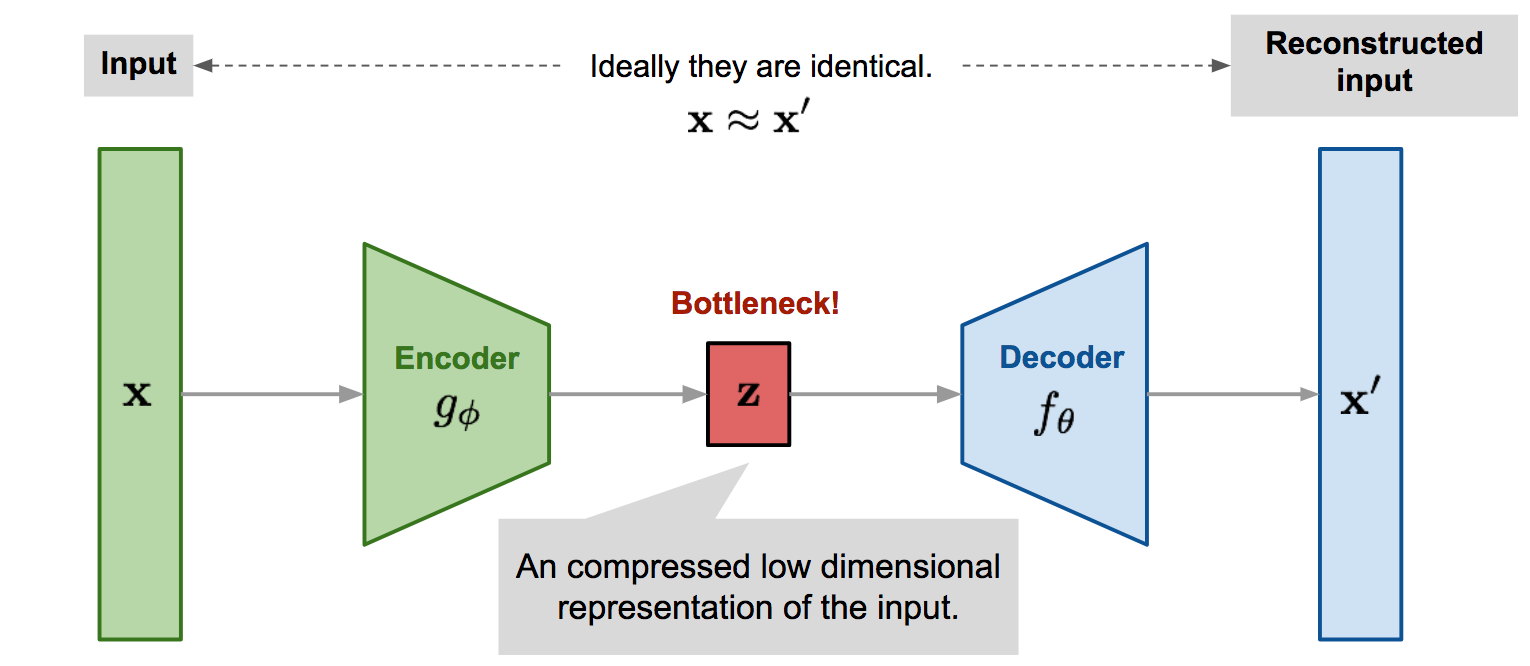
\includegraphics[width=1.0\linewidth]{imagenes/esquema_codificador.png}
	\caption{Esquema de la arquitectura empleada para inicializar el codificador y representación latente. \cite{subedi2022retracted}}
\end{figure}


El objetivo tras aplicar este esquema es construir un fuerte codificador que reduzca la dimensionalidad y una representación latente (bottleneck) que comprima las características principales de las imágenes del conjunto de entrenamiento.

En términos del proceso de optimización que es el entrenamiento, de forma no supervisada se están inicializando los pesos de la red para parecerse al conjunto de imágenes. \cite{zeiler2014visualizing} estudia como los diferentes filtros de las redes neuronales convolucionales al entrenarse ante una tarea de clasificación acaban replicando las características generales y específicas de las imágenes de las que son entrenados. Por ello, se llega a la conclusión de que una heurística importante dentro de las redes neuronales convolucionales es que \textbf{los filtros se parecen a las imágenes}. 

Esta razón explica de forma teórica como un proceso de ajuste previo al conjunto de entrenamiento elimina el coste computacional de búsqueda de los pesos via descenso del gradiente y backpropagation que require el ajuste de la red por sí misma a las imágenes sólo a partir de las etiquetas.

\subsection{Modelo de clasificación}

A continuación, presentamos el modelo de clasificación.

La entrada $x$ es el vector de características iniciales. En nuestro caso, son las tres imágenes correspondientes a las $3$ pruebas. El codificador es una red neuronal que transforma la entrada de alta dimensionalidad $x$ en una representación de menor dimensionalidad $z$. El proceso de codificación se puede ver como una función $g_{\phi}$ parametrizada por $\phi$, que aprende a extraer las características más relevantes de los datos de entrada. La parte final del esquema es una red neuronal densa que toma la representación comprimida $z$ y realiza la tarea específica del modelo

\begin{figure}[H]
	\centering
	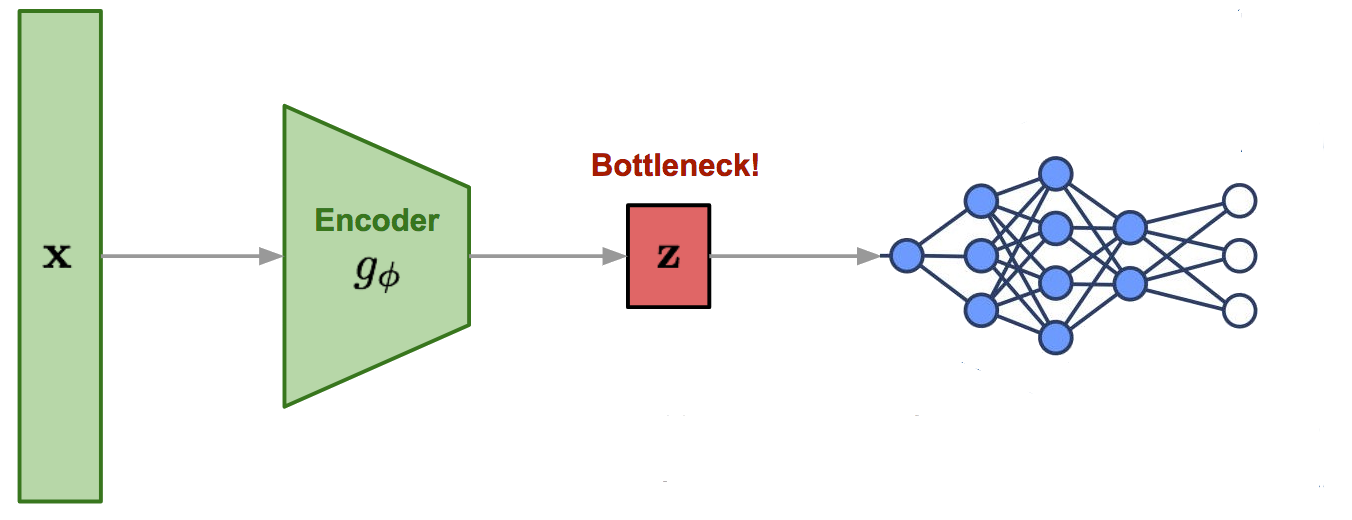
\includegraphics[width=0.9\linewidth]{imagenes/esquema_clasificacion.png}
	\caption{Esquema de la arquitectura empleada para el problema de clasificación}
\end{figure}

Tras ello tenemos un modelo capaz de distinguir entre las etiquetas \textbf{glioblastomas, meningiomas o no tumor} para imágenes donde aparecer uno de los esos dos tumores o no aparezca ninguno. Para transformarlo en un clasificación binaria para todas las imágenes de una resonancia aplicamos el siguiente esquema de votación.

\subsubsection{Esquema de votación}

Tras la salida de las neuronas en las $3$ etiquetas creadas para trabajar en 2D: \textbf{glioblastomas, meningiomas o no tumor}. Necesitamos una transformación de las predicciones individuales de cada imágenes a toda la resonancia. En la mayoría de los casos ante este tipo de problema se usa un \textbf{esquema de votación}.

Consideraremos un esquema de votación que utilice solo la cantidad de predicciones cuando exista tumor, es decir, cuando la etiqueta sea \textbf{Glioblastoma} o \textbf{Meningioma}. Mostraremos el esquema de votación que usamos en el siguiente pseudo-código.

\begin{algorithm}
	\caption{Predicción del tipo de tumor de toda la resonancia a partir de las predicciones de todas las imágenes de este}
	\begin{algorithmic}[1]
		\STATE \textbf{Function} \texttt{Votación}($Meningioma_{PREDS}$, threshold)
		\IF{$Meningioma_{PREDS} < threshold$}
		\STATE \textbf{return} "Meningioma"
		\ELSE
		\STATE \textbf{return} "Glioblastoma"
		\ENDIF
	\end{algorithmic}
\end{algorithm}

Tras este método sólo queda saber cual es el parámetro $threshold$ óptimo. Para ello, simplemente se ajustará a validación tras una búsqueda a través de fuerza bruta.

\subsection{Modelo de segmentación}

A continuación, presentamos el modelo para la tarea de segmentación. Muy similar al esquema para la reconstrucción tenemos un diferente y totalmente nuevo decodificador $S_{\sigma}$ especifico para la tarea de crear una máscara de segmentación. Se añaden conexiones (concatenaciones) entre el codificador y decodificador para poder preservar la precisión de las características de la imagen original. Finalmente la salida son las etiquetas $Y$ las cuales son las máscaras segmentación reales proporcionadas por \textbf{BraTS} y umbralizadas a toda la lesión tumoral.


\begin{figure}[H]
	\centering
	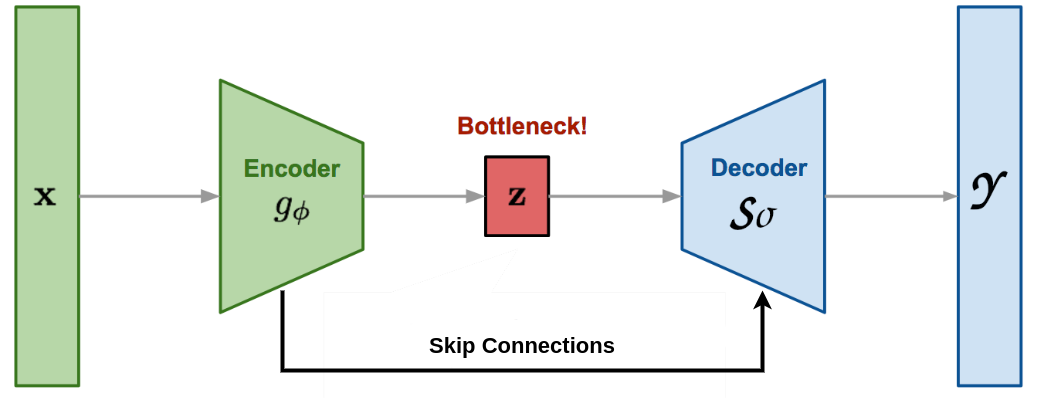
\includegraphics[width=0.9\linewidth]{imagenes/esquema_segmentacion.png}
	\caption{Esquema de la arquitectura empleada para el problema de segmentación}
\end{figure}

\subsection{Uso de transfer learning}

Dentro de las estrategias que podemos utilizar para una mayor convergencia en el aprendizaje y disminuir los tiempos de entrenamiento incluiremos el uso de \textbf{transfer learning}.

Debemos tener en cuenta que el entrenamiento en la tarea de la reconstrucción de las imágenes también es una estrategia de transfer learning, ya que transferimos el aprendizaje útil de la tarea de la reconstrucción a las tareas específicas del problema. Sin embargo, en esta sección nos enfocamos en usar transfer learning previamente a esa tarea. 

La única parte que usaremos de la arquitectura usada en el autoencoder será el codificador por tanto sólo nos preocupa el uso de transfer learning en esa parte de la red. En la búsqueda de un buen codificador $g_{\phi}$ podemos encontrar arquitecturas usadas en clasificación que capturan características visuales generales, de millones de imágenes diferentes. Es común para multitud de problemas el uso de arquitecturas previas entrenadas con el dataset \textbf{ImageNet}. 

Optamos por tomar como codificador una arquitectura previamente entrenada en este dataset, las arquitecturas candidatas que probaremos en el desempeño del problema serán: 

\begin{enumerate}
	\item \textbf{ResNet34}: Por su multitud de conexiones residuales reportadas en el estado del arte como factor positivo. Con una profundidad de 34 capas está entre sus arquitecturas hermanas ResNet18 y ResNet50 como una arquitectura no muy profunda que ofrece buen desempeño para variedad de problemas.
	
	\item \textbf{Xception}: A diferencia de \textbf{ResNet34} ofrece kernels de distinto tamaño que podrían favorecer la mejor caracterización de tumores de diferente tamaño. 
	
\end{enumerate}


\section{Diseño de las arquitecturas}

En el siguiente apartado detallaremos los módulos y capas que componen a las arquitecturas así como las componentes importantes. 

\subsection{Función de activación}

Para todas las arquitecturas (segmentación, clasificación y el autoencoder para construir el codificador), se optará por el uso de la función de activación ReLU (Rectified Linear Unit), definida como:

$$ \text{ReLU}(x) = \max(0, x) $$

Donde \( x \) es la entrada a la función ReLU.

A continuación, enunciamos algunas de las razones de su elección y su reconocida robustez para una gran amplitud de problemas en aprendizaje profundo.

\begin{enumerate}
	\item \textbf{No Linealidad:}
	ReLU introduce no linealidad en las redes neuronales, lo cual es crucial para que las redes puedan aprender y modelar relaciones y características complejas en los datos. Esta no linealidad es esencial para tareas como la clasificación y la segmentación, donde las relaciones entre los datos son inherentemente no lineales.
	
	\item \textbf{Gradiente Constante:}
	Para valores positivos de $ x $, la derivada de ReLU es constante e igual a 1. Esto evita el problema del desvanecimiento del gradiente en redes profundas, donde el gradiente puede volverse extremadamente pequeño en funciones de activación saturadas como la sigmoide y la tangente hiperbólica.
	
	\[ \frac{\partial \text{ReLU}(x)}{\partial x} = \begin{cases} 
		1 & \text{si } x > 0 \\
		0 & \text{si } x \leq 0 
	\end{cases} \]
	
	Esto facilita el entrenamiento de redes más profundas y la convergencia más rápida durante el proceso de optimización.
	
	\item \textbf{Eficiencia Computacional:}
	La función ReLU es eficiente en términos computacionales. Su implementación es simple (una comparación y una operación de máximo) y no involucra cálculos costosos como funciones exponenciales.
	
\end{enumerate}

La elección de ReLU como función de activación común a través de estas arquitecturas se basa en sus propiedades matemáticas que promueven la eficiencia, la no linealidad y la estabilidad del gradiente.

\subsection{Normalización por lotes}

Antes de aplicar la función de activación, aplicaremos \textbf{normalización por lotes}.
PyTorch que es la biblioteca que usaremos implementa la normalización por lotes descrita en \cite{ioffe2015batch}.

La normalización por lotes se aplica a la salida de una capa antes de aplicar la función de activación. Supongamos que tenemos una capa con activaciones $\mathbf{x}$, donde $\mathbf{x} \in \mathbb{R}^{m \times d}$, siendo $m$ el tamaño del lote y $d$ el número de características en cada ejemplo del lote.

Se calcula la media para cada característica a lo largo del lote:
\[
\mu_j = \frac{1}{m} \sum_{i=1}^{m} x_{ij}
\]
donde $\mu_j$ es la media de la característica $j$ y $x_{ij}$ es el valor de la característica $j$ del ejemplo $i$ en el lote.

Se calcula la varianza para cada característica a lo largo del lote:
\[
\sigma_j^2 = \frac{1}{m} \sum_{i=1}^{m} (x_{ij} - \mu_j)^2
\]
donde $\sigma_j^2$ es la varianza de la característica $j$.


Los datos se normalizan utilizando la media y la varianza calculadas:
\[
\hat{x}_{ij} = \frac{x_{ij} - \mu_j}{\sqrt{\sigma_j^2 + \epsilon}}
\]
donde $\hat{x}_{ij}$ es la característica $j$ del ejemplo $i$ normalizada, y $\epsilon$ es una pequeña constante (generalmente $10^{-5}$) para evitar la división por cero y mejorar la estabilidad numérica.


Después de la normalización, se aplica un escalamiento y un sesgo:
\[
y_{ij} = \gamma_j \hat{x}_{ij} + \beta_j
\]
donde $y_{ij}$ es la salida final para la característica $j$ del ejemplo $i$, $\gamma_j$ es un parámetro de escala aprendido, y $\beta_j$ es un parámetro de sesgo aprendido.

Durante el entrenamiento, tanto $\gamma_j$ como $\beta_j$ se optimizan junto con los otros parámetros de la red neuronal mediante el descenso de gradiente.

El uso de normalización por lotes tiene algunos \textbf{beneficios}.
\begin{itemize}
	\item \textbf{Estabilización del entrenamiento:} La normalización por lotes ayuda a reducir los problemas de desvanecimiento y explosión del gradiente, permitiendo que las redes neuronales más profundas se entrenen de manera más efectiva.
	\item \textbf{Regularización:} Actúa como una forma leve de regularización al introducir una varianza controlada en el proceso de entrenamiento, lo que a menudo conduce a una mejor generalización del modelo.
\end{itemize}


\subsection{Arquitectura para la reconstrucción de imágenes}

Como anunciábamos usamos una arquitectura bien conocida como codificador, probaremos la bondad de \textbf{ResNet34} y \textbf{Xception} en la experimentación. Tras ello, construimos un intuitivo espacio de capas que sean nuestra representación latente. 

\subsubsection{Arquitectura del codificador ResNet34}

A continuación, mostramos y comentamos la arquitectura de uno de los posibles codificadores que usaremos ResNet34.

La innovación clave de ResNet es el bloque residual, que introduce atajos o conexiones directas entre capas no adyacentes de la red. Estos bloques permiten que el flujo de información y los gradientes se propaguen directamente a través de la red, mitigando los problemas de desaparición y explosión del gradiente.

Un bloque residual típico se representa como:
$$ \mathbf{y} = \mathcal{F}(\mathbf{x}, \{W_i\}) + \mathbf{x} $$

Aquí, \(\mathbf{x}\) es la entrada del bloque, \(\mathcal{F}(\mathbf{x}, \{W_i\})\) es la transformación no lineal aprendida (que puede incluir capas como convoluciones, normalización y activaciones), y \(\mathbf{x}\) se suma a esta transformación para obtener la salida \(\mathbf{y}\). Esta suma es la conexión residual.

\begin{figure}[H]
	\centering
	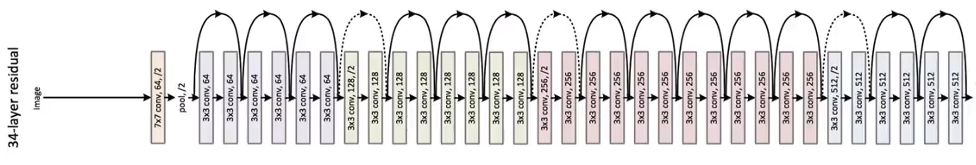
\includegraphics[width=1.0\linewidth]{imagenes/resnet34_arch.png}
	\caption{Arquitectura usada de ResNet34 \cite{he2016deep}}
\end{figure}

ResNet34 se compone de varias capas organizadas en bloques residuales. Como \textbf{capa de entrada} tiene una capa convolucional inicial con 64 filtros de tamaño 7x7 y un stride de 2, seguida de una capa de normalización y una capa de pooling de 3x3 con un stride de 2. Tras ello tenemos los siguientes \textbf{bloques residuales}:
\begin{itemize}
	\item 3 bloques con 64 filtros.
	\item 4 bloques con 128 filtros.
	\item 6 bloques con 256 filtros.
	\item 3 bloques con 512 filtros.
\end{itemize}

Cada bloque está compuesto por dos capas convolucionales de tamaño 3x3. Los bloques están organizados de manera que cada grupo de bloques de un determinado número de filtros tiene el mismo número de filtros a lo largo del grupo.

Como \textbf{capa final} después de todos los bloques residuales, se añade una capa de pooling global seguida de una capa completamente conectada (fully connected) que produce la salida final de la red. En este trabajo eliminamos esas dos capas finales para añadirle la representación latente.

\subsubsection{Arquitectura del codificador Xception}

A continuación, mostramos y comentamos la arquitectura de uno de los posibles codificadores que usaremos, \textbf{Xception}.

La arquitectura Inception, particularmente en sus versiones más recientes como Inception-v3, utiliza módulos Inception para capturar tanto características locales como globales en las imágenes. Sin embargo, estos módulos son complejos y pueden ser optimizados. Xception simplifica y mejora este diseño usando convoluciones separables en profundidad, lo que resulta en una red más eficiente y efectiva.

\begin{figure}[H]
	\centering
	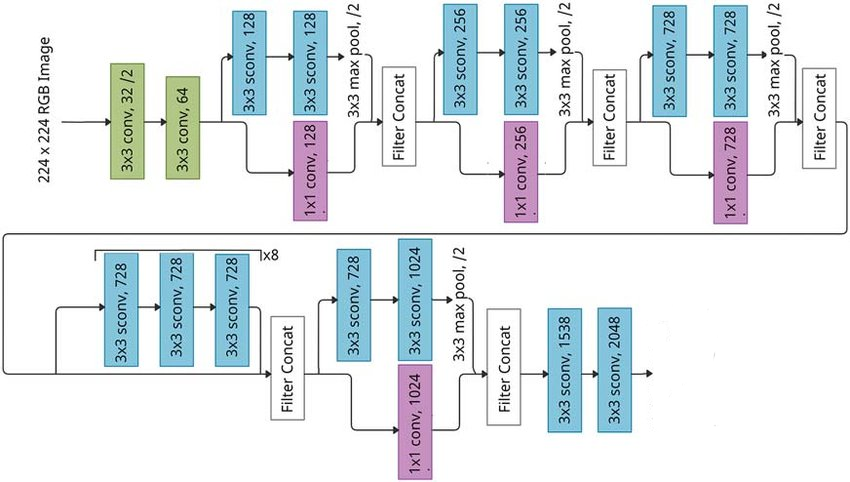
\includegraphics[width=0.8\linewidth]{imagenes/xception_arch.png}
	\caption{Arquitectura usada de Xception \cite{srinivasan2021performance}}
\end{figure}

La convolución separable en profundidad es una técnica que factoriza una convolución estándar en dos operaciones más simples y eficientes: una \textbf{convolución en profundidad} (depthwise convolution) y una \textbf{convolución puntual} (pointwise convolution). En una convolución estándar, los filtros de convolución mezclan canales de entrada y espaciales en una única operación. En cambio, la convolución separable en profundidad realiza estos dos pasos por separado.

Matemáticamente, una convolución separable en profundidad donde \(\mathbf{X}\) es la entrada, \(\mathbf{K}\) es el filtro de convolución, \(*_{\text{depthwise}}\) es la operación de convolución en profundidad y \(*_{\text{pointwise}}\) es la operación de convolución puntual.

Xception se compone de varias capas organizadas en bloques de convolución separables en profundidad. Como capa de entrada tiene una capa convolucional inicial con 32 filtros de tamaño 3x3 y un stride de 2, seguida de una capa convolucional con 64 filtros de tamaño 3x3.

\begin{itemize}
	\item \textbf{Entrada al módulo}: Tres bloques con convoluciones separables en profundidad con 128, 256 y 728 filtros respectivamente.
	\item \textbf{Módulos intermedios}: Ocho bloques idénticos con convoluciones separables en profundidad con 728 filtros cada uno.
	\item \textbf{Salida del módulo}: Tres bloques con convoluciones separables en profundidad con 728, 1024 y 1536/2048 filtros respectivamente.
\end{itemize}

Cada bloque de convolución separable en profundidad consiste en una convolución en profundidad seguida de una convolución puntual y una capa de activación ReLU.

Al igual que \textbf{ResNet34} en la arquitectura original se añade una capa de pooling global seguida de una capa completamente conectada (fully connected) que produce la salida final de la red. Sin embargo, nosotros eliminamos esas capas y le conectamos la representación latente.

\subsubsection{Espacio de capas de la representación latente y bloque ConvBlock}

A continuación, describiremos qué capas y dimensiones tiene la representación latente. Para todas las tareas (clasificación y segmentación) al igual que el codificador se compartirá la misma representación latente. Podemos ver la arquitectura de la representación latente en un diagrama.

\begin{figure}[H]
	\centering
	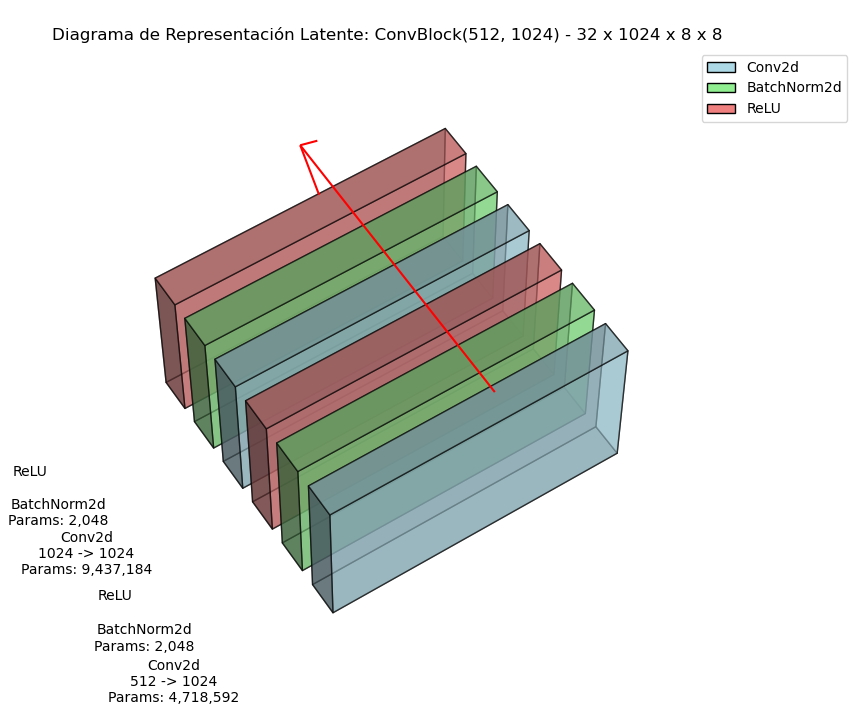
\includegraphics[width=0.8\linewidth]{imagenes/bottleneck_arch.png}
	\caption{Arquitectura de la representación latente}
\end{figure}

El bloque \textbf{ConvBlock(512, 1024)} se utiliza como representación latente dentro de nuestro autoencoder representa una etapa de procesamiento que transforma una entrada de 512 canales (o características) en una salida de 1024 canales mediante operaciones convolucionales seguidas de normalización y activación no lineal. En detalle, el bloque consiste de dos capas convolucionales cada una seguida por capas de Batch Normalization y activación ReLU. La primera capa convolucional transforma los 512 canales de entrada en 1024 canales de salida, manteniendo el tamaño de la entrada con un kernel de 3x3, stride de 1 y padding de 1. Luego, la segunda capa convolucional opera sobre los 1024 canales de salida, manteniendo este número de canales con el mismo tamaño de kernel y configuración de stride y padding. La capa de Batch Normalization se aplica después de cada capa convolucional para estabilizar y acelerar el entrenamiento, y la ReLU como función de activación introduce no linealidades que ayudan a capturar características más complejas en los datos de entrada. Este tipo de bloque que funciona como representación latente del conjunto de datos, es crucial en redes autoencoder para aprender representaciones más profundas y significativas de los datos, condensando y expandiendo la información a través de capas convolucionales apiladas.

\subsubsection{Reducción de canales}

Ambas arquitecturas que probaremos \textbf{ResNet34} y \textbf{Xception} están inicialmente pensadas para imágenes a color, es decir, imágenes en RGB que contenga tres canales o capas pertenecientes a cada tonalidad de colores primarios. Intuitivamente y apoyado por el estado del arte una simple forma de manejar las pruebas para construir una entrada a la red es \textbf{concatenarlas}. De esta forma, una entrada a la red estaría compuesta de una imagen de cuatro canales (uno por tipo resonancia que tenemos o prueba), en otras palabras cuatro imágenes en escala de grises concatenadas respecto un eje $Z$ que representaría la profundidad del volumen de la entrada.


Sin embargo, las arquitecturas empleadas como codificador sólo aceptan imágenes de tres canales. Para lidiar con ello se plantea una reducción de dimensionalidad para transformar las imágenes de cuatro canales a tres canales. A nivel práctico se plantea llevarse a cabo mediante:

\begin{enumerate}
	\item \textbf{Transformación mediante análisis de componentes principales PCA a las tres componentes principales}. Se plantea como la mejor solución de las dos que exploraremos ya que se reduce la información manteniendo la mayor variabilidad posible tras combinar linealmente las imágenes. 
	
	Podemos apreciar como la imagen de una resonancia es transformada con PCA dando la siguiente salida.
	
	\begin{figure}[H]
		\centering
		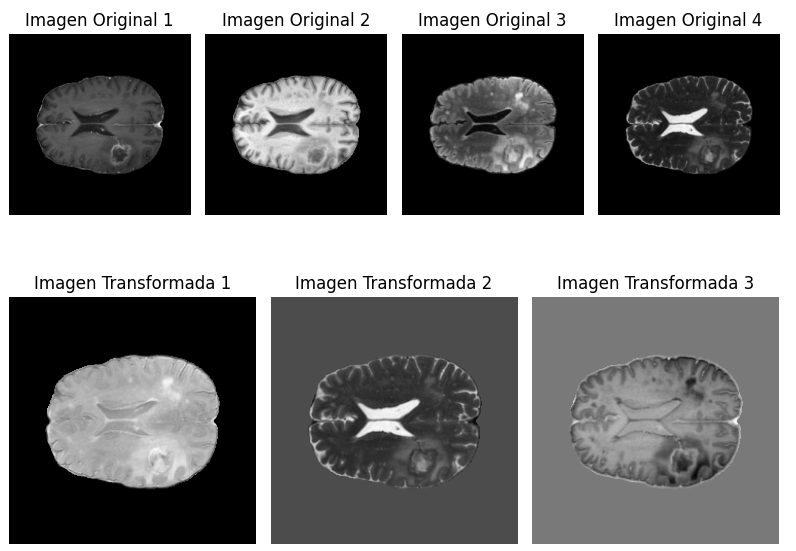
\includegraphics[width=0.8\linewidth]{imagenes/PCA_reduction.png}
		\caption{Ejemplo de transformación mediante PCA}
	\end{figure}
	
	Para aplicar PCA podemos optar por diferentes estrategias atendiendo si queremos incluirlo o no como una más del preprocesamiento de datos.
	
	\begin{enumerate}
		\item \textbf{Mediante el preprocesamiento de todo el conjunto de datos aplicando PCA}. Se puede preprocesar los datos y subirlos a Kaggle de nuevo. Sin embargo, esta opción no se pudo aplicar en la práctica debido a las limitaciones de espacio en disco que nos daba la plataforma.
		
		\item \textbf{Mediante la aplicación de PCA en el mismo entrenamiento antes de introducirlo a la red}. Esta opción elimina la sobrecarga en memoria en disco de Kaggle pero en la práctica es rápidamente descartada ya que aumenta $\approx 50 \%$ el tiempo en entrenamiento. Esta implicación teniendo una limitación de tiempo en Kaggle muy ajustada no la hacen compatible con un entrenamiento completo.
	\end{enumerate}
	
	\item \textbf{Eliminación de una prueba}. Una solución más agresiva es la propia eliminación de un canal de entre los originales. Las principales ventajas de esta solución es la gran facilidad para aplicarla y la mejora del tiempo de extracción de las imágenes puesto ya ahorraríamos traer la eliminada mejorando un $25 \%$ los tiempos de extracción de disco. 
	
	Ante la imposibilidad de aplicar PCA se aplicará esta segunda solución. Se elige eliminar a las imágenes de las resonancias de tipo \textbf{T2W} por ajuste al problema. Se descarta la eliminación de la información con y sin agente de contraste que proporcionan las tipo T1. Entre la elección de \textbf{T2F} y \textbf{T2W} la diferencia principal entre las dos es que en la de tipo \textbf{T2W} el líquido cefalorraquídeo contrasta. En toda la revisión médica del problema no se indica que sea un factor relevante en la segmentación de tumores cerebrales por lo que se conserva a la de tipo \textbf{T2F} que mantiene una imagen más nítida al no contrastar con el líquido cefalorraquídeo.
	
\end{enumerate}

\subsubsection{Bloque UpConv}

Con el objetivo de describir la parte decodificadora de la arquitectura vamos a definir nuestro propio bloque \textbf{UpConv}. Definimos el bloque UpConv como una operación de convolución transpuesta seguido de la aplicación del bloque \textbf{ConvBlock} definido en el apartado de la representación latente.

La \textbf{operación de convolución transpuesta o deconvolución} se define como la inversa de la convolución estándar en una red neuronal convolucional. A continuación, se explica los detalles matemáticos de la convolución transpuesta.

\begin{enumerate}
	\item \textbf{Entrada}: Sea \( x \in \mathbb{R}^{C_{in} \times H_{in} \times W_{in}} \), donde \( C_{in} \) es el número de canales de entrada, y \( H_{in}, W_{in} \) son la altura y anchura de la entrada, respectivamente.
	
	\item \textbf{Salida}: Sea \( y \in \mathbb{R}^{C_{out} \times H_{out} \times W_{out}} \), donde \( C_{out} \) es el número de canales de salida, y \( H_{out}, W_{out} \) son la altura y anchura de la salida, respectivamente.
\end{enumerate}

La operación de convolución transpuesta aplica un kernel de convolución de tamaño \( (k_{H}, k_{W}) \) sobre la entrada \( x \), utilizando un paso (stride) \( s \) y un relleno (padding) \( p \). En nuestro caso, siendo siempre constante $p = 0$ y $s = 2$ La operación se define de la siguiente manera:

\[
H_{out} = (H_{in} - 1) \cdot s - 2p + k_{H}
\]
\[
W_{out} = (W_{in} - 1) \cdot s - 2p + k_{W}
\]

Número de canales de salida: \( C_{out} \)

Sea \( w \in \mathbb{R}^{C_{out} \times C_{in} \times k_{H} \times k_{W}} \) el kernel de la convolución transpuesta.

Para cada posición \( (h', w') \) en la salida:
\[
y_{c}(h', w') = \sum_{c'=1}^{C_{in}} \sum_{h=0}^{k_{H}-1} \sum_{w=0}^{k_{W}-1} w_{c,c',h,w} \cdot x_{c'}(h' \cdot s + h - p, w' \cdot s + w - p)
\]

donde \( y_{c}(h', w') \) es el elemento en la posición \( (h', w') \) del canal \( c \) de la salida \( y \), \( x_{c'} \) es el elemento en la posición correspondiente en el canal \( c' \) de la entrada \( x \), y \( w_{c,c',h,w} \) es el peso del kernel en la posición \( (c, c', h, w) \).

El principal objetivo de la deconvolución es aumentar las dimensiones espaciales de la imagen de entrada, permitiendo reconstruir información espacialmente más detallada a partir de las características aprendidas. De esta forma, el decoder puede reconstruir las imágenes o máscaras a partir de la reducción de las imágenes entrada a la red. 

\subsubsection{Decodificador}

Construimos el decodificador como la secuencia de cuatro bloques \textbf{UpConv}. En este caso, para la primera tarea de reconstrucción con entradas y salidas: (1024, 512), (512, 256), (256, 128), (128, 64). 

\subsection{Arquitectura para clasificación}

Tras la construcción de la arquitectura para reconstrucción ya tendríamos listos el codificador y la representación latente. Para resolver el problema de clasificación creamos la siguiente arquitectura.

\begin{figure}[H]
	\centering
	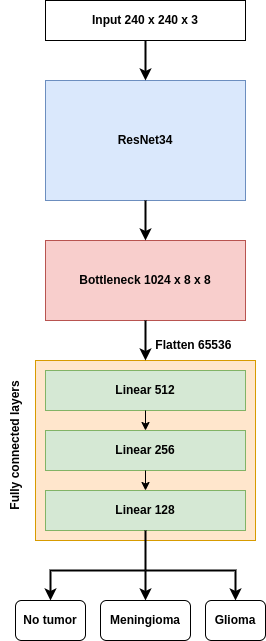
\includegraphics[width=0.3\linewidth]{imagenes/arquitectura_clasificacion.png}
	\caption{Arquitectura para la tarea de clasificación}
\end{figure}

Utilizamos el codificador seguido de la representación latente tras la representación latente aplanamos su salida con una capa \textbf{Flatten} para ahora solo quedará reducir esta salida a $3$ neuronas mediante la aplicación de varias capas de neuronas densamente conectadas. En concreto, $3$ capas con $512$, $256$ y $128$ neuronas hasta la capa final de $3$ neuronas de la que tomamos su máxima neurona como salida.

\subsection{Arquitectura para segmentación}

Tras construir la arquitectura autoencoder para el problema de la reconstrucción, adaptarla para el problema de segmentación es una tarea sencilla. Por un lado, observamos como la estadarización que presentan los datos es favorable para que una misma arquitectura (en el contexto que es una red con unas dimensiones y capas fijas) sea igualmente apta en ambos problemas (reconstrucción y segmentación). Si recordamos \cite{myronenko20193d} utilizaba esta idea, su arquitectura de doble tarea comparte codificador y representación latente, y además ambos decodificadores son prácticamente idénticos. Por lo tanto, se mantendrá el mismo diseño de decodificador que en la tarea de la reconstrucción. La única diferencia que se introducirá en segmentación será el uso de \textbf{skips connections}.

\subsubsection{Skips connections} 

Con la inclusión de \textbf{Skips connections} la arquitectura para la tarea de segmentación se convierte en una variante de una arquitectura ampliamente conocida, la \textbf{U-net} \cite{ronneberger2015u}. Las similitudes que comparte la arquitectura propuesta con ella es que los decoder de ambas arquitecturas son iguales y se tiene el mismo número de Skips connections. 

Sin embargo, a diferencia de la U-net que mantiene una simetría en dimensiones entre encoder y decoder, tanto ResNet34 como Xception son un encoder más profundos que el encoder de la U-net original rompiendo la simetría en la arquitectura propuesta. Por otro lado, ambos contienen conexiones residuales transformando la arquitectura en una variante llamada \textbf{Residual U-net} o \textbf{ResU-net}. 

A continuación, mostramos en un diagrama la arquitectura para la tarea de segmentación.

\begin{figure}[H]
	\centering
	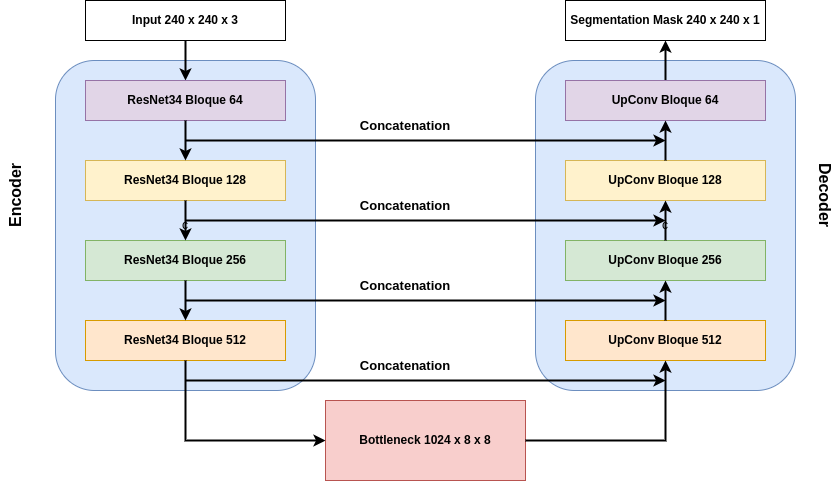
\includegraphics[width=1.0\linewidth]{imagenes/arquitectura_segmentacion.png}
	\caption{Arquitectura para la tarea de segmentación}
\end{figure}

Podemos ver como representamos a las skip connections como una simple concatenación de igual que forma que pasaba en las conexiones residuales pero de forma más general concatenando la salida de un módulo (grupo de capas) con la entrada de este.  


\section{Optimización de las arquitecturas}

En la siguiente sección detallaremos las funciones de pérdida usadas en cada arquitectura y la metodología seguida para llevar a cabo el entrenamiento de la red.

\subsection{Optimizador}

En este trabajo usaremos al optimizador por defecto de \textbf{Fastai}, \textbf{Adam}. El optimizador \textbf{Adam} (Adaptive Moment Estimation) \cite{kingma2014adam} es uno de los métodos de optimización más populares utilizados en el entrenamiento de redes neuronales profundas. Combina las ventajas de otros dos métodos conocidos: AdaGrad y RMSProp, ofreciendo una optimización más eficiente.

Adam ajusta los parámetros de la red neuronal basándose en el promedio de los gradientes y el promedio de los cuadrados de los gradientes. Los pasos principales que sigue son los siguientes:

\begin{enumerate}
	\item \textbf{Gradiente:} En cada iteración del entrenamiento, Adam calcula el gradiente de la función de pérdida con respecto a los parámetros del modelo. El gradiente indica la dirección y magnitud en la que los parámetros deben ajustarse para reducir la pérdida.
	
	\item \textbf{Promedio de gradientes (primer momento):} Adam calcula un promedio móvil de los gradientes. Esto ayuda a suavizar los cambios bruscos en la dirección del gradiente, proporcionando una dirección más estable para la actualización de los parámetros.

	$$ m_t = \beta_1 m_{t-1} + (1 - \beta_1) g_t $$

	donde $m_t$ es el promedio móvil de primer momento, $g_t$ es el gradiente en el tiempo $t$, y $\beta_1$ es el coeficiente de decaimiento exponencial para los promedios de primer momento.
	
	\item \textbf{Promedio de cuadrados de gradientes (segundo momento):} Adam también calcula un promedio móvil de los cuadrados de los gradientes. Esto permite ajustar la tasa de aprendizaje para cada parámetro individualmente, reduciendo la tasa de aprendizaje para los parámetros con gradientes grandes y aumentando la tasa para los parámetros con gradientes pequeños.

	$$ v_t = \beta_2 v_{t-1} + (1 - \beta_2) g_t^2 $$

	donde $v_t$ es el promedio móvil de segundo momento, $g_t$ es el gradiente en el tiempo $t$, y $\beta_2$ es el coeficiente de decaimiento exponencial para los promedios de segundo momento.
	
	\item \textbf{Corrección de sesgo:} Al principio del entrenamiento, los promedios móviles pueden estar sesgados hacia cero. Adam corrige este sesgo para obtener estimaciones más precisas de los promedios.

	$$ \hat{m}_t = \frac{m_t}{1 - \beta_1^t} $$

	$$ \hat{v}_t = \frac{v_t}{1 - \beta_2^t} $$

	
	\item \textbf{Actualización de parámetros:} Finalmente, Adam ajusta los parámetros del modelo utilizando los promedios móviles corregidos.

	$$ \theta_t = \theta_{t-1} - \frac{\alpha \hat{m}_t}{\sqrt{\hat{v}_t} + \epsilon} $$

	donde $\theta_t$ son los parámetros del modelo en el tiempo $t$, $\alpha$ es la tasa de aprendizaje, y $\epsilon$ es un pequeño valor para evitar la división por cero.
\end{enumerate}

\subsection{Funciones de pérdida}

En este apartado detallamos las funciones de pérdida utilizadas en las diferentes tareas.

\subsubsection{Función de pérdida para la reconstrucción de imágenes}

Usamos el \textbf{error absoluto medio} (MAE) de los píxeles de salida reconstruidos y los verdaderos como función de pérdida para realizar la reconstrucción de las imágenes. El MAE mide la magnitud promedio de las diferencias absolutas entre los valores predichos por el modelo y los valores reales. Esta métrica es útil para evaluar la precisión de la reconstrucción de las imágenes, ya que considera todas las diferencias de manera uniforme, sin penalizar más las diferencias grandes que las pequeñas.

$$ \text{MAE} = \frac{1}{n} \sum_{i=1}^{n} \left| y_i - \hat{y}_i \right| $$ 

Donde $n$ es el número total de píxeles en la imagen, $y_i$ es el valor verdadero del píxel $i$ y $\hat{y}_i$ es el valor reconstruido o predicho del píxel $i$.

En el contexto de la reconstrucción de imágenes, cada $y_i$ representa la intensidad del píxel en la imagen original, y cada $\hat{y}_i$ representa la intensidad del píxel en la imagen reconstruida por el modelo. El MAE proporciona una medida directa de cuán cerca están las intensidades de los píxeles reconstruidos de las intensidades reales.

También usaremos la misma pérdida como métrica de bondad de ajuste del modelo. Esto significa que, además de utilizar el MAE para optimizar el modelo durante el entrenamiento, también lo emplearemos para evaluar el desempeño del modelo en la reconstrucción de imágenes. Utilizar el MAE como métrica de evaluación nos permite tener una interpretación clara y consistente de cómo de bien se está desempeñando el modelo en términos de error promedio de los píxeles reconstruidos.

\subsubsection{Función de pérdida para clasificación}

Focal Loss es una función de pérdida que se ha demostrado ser particularmente efectiva para problemas de clasificación, especialmente en contextos donde hay un desequilibrio en las clases o cuando algunas muestras son más difíciles de clasificar que otras. Tras el procesamiento de datos, no existe un desbalanceo de datos grande. Sin embargo, la naturaleza de los tumores hacen que existan imágenes muy variables entre sí (con distinto grado de dificultad de optimización) es por ello que se opta por una pérdida que tenga algún mecanismo de control sobre esto. A continuación se explica por qué la Focal Loss puede ser mejor que la tradicional Cross Entropy Loss, especialmente en el contexto de datos con diferentes niveles de dificultad:

La Cross Entropy Loss es la función de pérdida estándar para problemas de clasificación y se define como:
$$  {\text{CE}} = - y_i \log(p_i) $$
$$  L_{\text{CE}} = - \sum_{i=1}^N y_i \log(p_i) $$

donde $y_i$ es la etiqueta verdadera y $p_i$ es la probabilidad predicha de la clase correcta. Aunque es efectiva, tiene algunas limitaciones:
\begin{enumerate}
	\item \textbf{Tratamiento Igualitario de todos los ejemplos}: Cross Entropy Loss trata todos los ejemplos de entrenamiento por igual, sin importar si son fáciles o difíciles de clasificar.
	\item \textbf{Sensibilidad al desbalanceo de clases}: No maneja bien los datos desbalanceados, donde algunas clases son mucho más frecuentes que otras.
\end{enumerate}

Focal Loss, propuesta por \cite{lin2017focal}, introduce un término adicional para enfocar el entrenamiento en ejemplos más difíciles. Se define como:

$$ {\text{FL}} = - \alpha (1 - p_t)^\gamma \log(p_t) $$
$$ L_{\text{FL}} = - \sum_{i=1}^N \alpha_t (1 - p_{t_i})^\gamma \log(p_{t_i})$$

donde $p_t$ es la probabilidad predicha de la clase correcta, $\alpha$ es un factor de ponderación para balancear la importancia de las clases, y $\gamma$ es el parámetro de focalización. Se puede desarrollar su principal ventaja:

\begin{enumerate}
	\item \textbf{Enfoque en ejemplos difíciles}: El término $(1 - p_t)^\gamma$ reduce la pérdida para los ejemplos bien clasificados (donde $p_t$ es alto) y mantiene alta la pérdida para los ejemplos mal clasificados (donde $p_t$ es bajo).
	
	\begin{enumerate}
		\item Cuando un ejemplo es fácil de clasificar ($p_t$ es alto), el término $(1 - p_t)^\gamma$ es pequeño, reduciendo su contribución a la pérdida total.
		\item Cuando un ejemplo es difícil de clasificar ($p_t$ es bajo), el término $(1 - p_t)^\gamma$ es grande, incrementando su contribución a la pérdida total.
	\end{enumerate}
	
	\item \textbf{Parámetro de Focalización}: El parámetro $\gamma$ ajusta el grado de focalización. Con $\gamma=0$, Focal Loss se reduce a la Cross Entropy Loss. Valores más altos de $\gamma$ incrementan el enfoque en los ejemplos difíciles.
	
	\item \textbf{Reducción del impacto de ejemplos fáciles}: Dado que los ejemplos fáciles no dominan el gradiente debido al término de focalización, el modelo no se sesga hacia las clases dominantes o los ejemplos que ya son bien clasificados.
	
\end{enumerate}

Esto implica los siguientes beneficios cuando existen datos de diferente dificultad.

\begin{enumerate}
	\item \textbf{Mejora del rendimiento general}: En muchos problemas de clasificación, hay ejemplos que son intrínsecamente difíciles de clasificar debido a la superposición de clases, ruido en los datos, o características ambiguas. Focal Loss ayuda a mejorar el rendimiento general del modelo al hacer que el modelo preste más atención a estos ejemplos difíciles durante el entrenamiento.
	
	\item \textbf{Mejor manejo de outliers}: Al reducir la contribución de ejemplos fáciles a la pérdida total, Focal Loss puede ayudar a mitigar el impacto de outliers o ejemplos atípicos que podrían desviar el modelo cuando se usa Cross Entropy Loss.
	
	\item \textbf{Robustez en modelos de gran escala}: En problemas similares como la detección de objetos en imágenes, donde el desequilibrio entre fondo y objeto puede ser significativo y algunos objetos son más difíciles de detectar que otros, Focal Loss ha demostrado ser particularmente útil.
	
\end{enumerate}

Focal Loss es una mejora sobre Cross Entropy Loss al proporcionar un mecanismo para enfocarse en ejemplos díficiles tales como imágenes donde los tumores sean pequeños. Con la gran en este problema de que realmente no queremos principalmente predecir muy bien la mayoría de ejemplos sino ser precisos en los ejemplos especialmente difíciles también para el personal médico. Por todo ello, se opta por utilizar \text{Focal Loss} para la primera tarea de clasificación.

\subsubsection{Función de pérdida para segmentación}

Como función de pérdida en segmentación se escoge el complemento negativo de su métrica más importante \textbf{similaridad Dice}: \textbf{Dice Loss}. Dice Loss se define como:

$$ L_{dice} = 1 - Dice(A, B) $$

Por lo tanto,  \textbf{Dice Loss} varía entre 0 y 1, donde 0 indica una superposición perfecta y 1 indica ninguna superposición (es decir, pérdida máxima).

Podemos enumerar las características que hacen de Dice Loss una de las pérdida más acertadas para la segmentación de tumores cerebrales. 

\begin{enumerate}
	\item \textbf{Sensibilidad a pequeñas áreas}: En la segmentación de tumores cerebrales, es crucial detectar incluso pequeñas regiones de tumores. El Dice Loss está diseñado para ser sensible a estas pequeñas áreas de superposición, lo que permite que el modelo se entrene para identificar y segmentar con precisión los bordes y áreas menos visibles del tumor.
	
	\item \textbf{Interpretabilidad clínica directa}: El coeficiente de similaridad Dice, en el que se basa el Dice Loss, proporciona una medida directa de cuán bien la predicción del modelo coincide con la realidad clínica. Esta métrica es intuitiva para los profesionales de la salud, ya que refleja la precisión de la segmentación en términos de superposición de áreas tumorales detectadas.
	
	\item \textbf{Robustez ante desbalanceo en la distribución de clases}: Los tumores cerebrales pueden representar solo una pequeña fracción de la imagen total, lo que genera desequilibrios en la distribución de clases. Dice Loss maneja este desequilibrio al penalizar menos la falta de predicción en áreas dominadas por el tejido cerebral normal, centrándose en mejorar la detección precisa de los tumores.
	
	\item \textbf{Optimización efectiva en el entrenamiento}: El uso de Dice Loss proporciona una superficie de optimización más suave y estable durante el entrenamiento de modelos de segmentación que otras pérdidas. Esto facilita la convergencia del modelo y reduce la necesidad de ajustes complejos de hiperparámetros, mejorando así la eficiencia del entrenamiento y la calidad de las segmentaciones obtenidas.
\end{enumerate}


\subsection{One-Cycle Policy}

La \textbf{política 1cycle} fue propuesta por \cite{smith2019super}, y es una técnica de programación de tasas de aprendizaje para mejorar el rendimiento del entrenamiento de redes neuronales. El objetivo principal es encontrar tasas de aprendizaje que aceleren el entrenamiento y mejoren la generalización del modelo. También ajusta la tasa de aprendizaje durante el entrenamiento de manera específica en función del número de iteraciones. Esta utiliza un ciclo de entrenamiento único en lugar de tasas de aprendizaje fijas durante todo el entrenamiento. Durante este ciclo, la tasa de aprendizaje varía de manera cíclica desde un valor inicial hasta un valor máximo y luego vuelve a descender.

En la primera mitad del ciclo, la tasa de aprendizaje aumenta gradualmente desde un valor inicial hasta un valor máximo. Este aumento permite una exploración más rápida del espacio de parámetros y puede ayudar a escapar de mínimos locales subóptimos. En la segunda mitad del ciclo, la tasa de aprendizaje disminuye gradualmente desde el valor máximo hasta el valor inicial. Esto permite una refinación más precisa de los pesos del modelo y una convergencia más estable hacia el mínimo global.

Además de ajustar la tasa de aprendizaje, la política 1cycle también propone variar el \textbf{momentum} (una técnica que ayuda a acelerar el entrenamiento). El momentum se incrementa en la fase de aumento y disminuye en la fase de descenso.

La política 1cycle también actúa como una forma de regularización. El uso de tasas de aprendizaje más altas en la fase de aumento y más bajas en la fase de descenso puede ayudar a prevenir el sobreajuste. También sugiere seleccionar los valores iniciales y máximos de la tasa de aprendizaje de manera específica. El valor máximo de la tasa de aprendizaje se elige típicamente como un valor que es varias veces mayor que el valor inicial. 

La duración total del ciclo puede variar, pero en general, se sugiere que sea aproximadamente igual al número total de épocas de entrenamiento.
La \textbf{política 1cycle} ha demostrado ser efectiva en mejorar la convergencia y la generalización en una variedad de tareas y arquitecturas de redes neuronales. Sin embargo, la selección precisa de los parámetros, como las tasas de aprendizaje inicial y máxima requiere ajustes específicos para cada objetivo y conjunto de datos.

En el uso conjunto de una política de \textbf{1cycle} y el optimizador \textbf{Adam} como se aplica en este trabajo, podemos entender como \textbf{1cycle} ajustaría la tasa de aprendizaje para una misma época (una tasa de aprendizaje global a una época) y Adam más tarde la refinaría ligeramente para cada ejemplo dentro de una época.  

En este trabajo usaremos esta política como forma de regularización y como método general para evitar la búsqueda de hiperparámetros manual para el proceso de aprendizaje. Para ello, en todo el trabajo sólo usaremos las llamadas a las funciones \texttt{fit\_one\_cycle()} para entrenar toda las capas de la red y \texttt{fine\_tune()} para cuando necesitemos diferenciar qué épocas entrenar toda la red (incluyendo la parte convolucional) o solo la parte densamente conectada. Ambas funciones son de la librería \textbf{Fastai} que implementan la política 1cycle. 

\section{Evaluación y métricas}

Para la evaluación se distinguirán entre tres subconjuntos de datos: entrenamiento, validación y test. Se utilizará un conjuntos fijos basado en \textbf{hold out}, común a todas las tareas. Por motivos de eficiencia no podemos permitirnos usar validación cruzada o distintos conjuntos variables. Estos conjuntos serán separados mediante la utilización de archivos CSV con las rutas absolutas de cada ejemplo para cada uno de ellos. 

Seguirán la siguiente distribución: un $49 \%$ para entrenamiento, $21 \%$ para validación y un $30 \%$ para test del conjunto total de datos (glioblastomas y meningiomas juntos) haciendo un reparto aleatorio entre ellos. Se sigue la regla de partición: $70 \%$ entrenamiento + validación y $30 \%$ test. La finalidad de cada subconjunto es para entrenamiento ajustar los modelos a este subconjunto de datos, el objetivo del conjunto de validación es elegir el mejor modelo de los probados, y el conjunto de test dar el resultado final garantizador de la bondad de los modelos.

\subsection{Métricas para clasificación}

Las métricas que vamos a usar para el proceso de clasificación son \textbf{accuracy balanceado} y \textbf{accuracy} que podremos calcular a través de la construcción de la matriz de confusión. 

\begin{enumerate}
	\item \textbf{Accuracy.} Mide cuántas predicciones del modelo son correctas respecto el total del predicciones. Se calcula como: 
	
	$$ \text{Accuracy} = \frac{\text{Nº de predicciones correctas}}{\text{Total de predicciones}} = \frac{TP + TN}{TP + TN + FP + FN}$$
	
	\item \textbf{Accuracy balanceado.} Esta métrica se usa en problemas de clasificación para manejar conjuntos de datos desbalanceados, donde las clases no están igualmente representadas. Se define como el promedio de las tasas de acierto (recall) obtenidas en cada clase, lo que ayuda a proporcionar una evaluación más justa y equilibrada del desempeño del modelo cuando las clases tienen diferentes tamaños.
	
	De forma general para un problema de clasificación de $N$ clases se calcula como:
	
	$$  \text{Balanced Accuracy} = \frac{1}{N} \sum_{i=1}^{N} \frac{TP_i}{TP_i + FN_i}$$
	
	De forma específica, para clasificación binaria $N = 2$ podemos expresarlo como:
	
	$$ \text{Balanced Accuracy} = \frac{1}{2} \left( \frac{TP}{TP + FN} + \frac{TN}{TN + FP} \right) $$ 
\end{enumerate}


\subsection{Métricas para segmentación}

Siguiendo la definición de evaluación de \textbf{BraTS} 2023, la evaluación de los tumores en su forma original comprende la segmentación de tres zonas diferenciadas según los tipos de tejidos que hay en ella. En \textbf{BraTS} se estudian los siguientes tres conjuntos de tejidos tumoral.

\begin{enumerate}
	\item \textbf{Enhancing Tumor ET}: Sólo incluye al tejido ET.
	\item \textbf{Tumor Core TC}: Incluye al tejido ET y al tejido NCR.
	\item \textbf{Whole Tumor WT}: Incluye a todos los tejidos enfermos: ET, NCR y ED. La segmentación de toda la lesión.
\end{enumerate}

Sin embargo, en este trabajo hacemos una reducción del problema por falta de recursos a \textbf{la segmentación únicamente del conjunto WT Whole Tumor}. De esta forma, la misión que tendremos es la de segmentar tejido enfermo o lesionado en todo el volumen de la resonancia. En otras palabras, diferenciar con la segmentación el tejido enfermo del tejido sano o la no existencia de tejido.

Para ello, se utilizará tres métricas. Las dos primeras utilizadas en todas las competiciones de \textbf{BraTS} y la tercera adicionalmente utilizada en los trabajos que han ido conformando el estado del arte como \cite{zhou2021latent}.

\begin{enumerate}
	\item \textbf{Similaridad Dice} : Mide la similaridad de dos conjuntos a través de la intersección de ambos respecto el tamaño total de los dos conjuntos.
	
	\begin{figure}[!h]
		\centering
		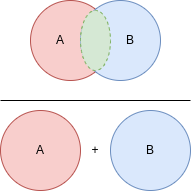
\includegraphics[width=0.25\linewidth]{imagenes/dicesimilarity.drawio.png}
		\caption{Interpretación del coeficiente de Similaridad Dice}
	\end{figure}
	
	Podemos expresarlo como:
	
	$$ Dice(A, B) = \frac{2 \times |A \cap B|}{|A| + |B|}$$
	
	Donde $A$ es la segmentación que proporcionará nuestro modelo y $B$ la verdadera.
	
	De forma más detallada, para una resonancia completa podemos expresarlo como:
	
	$$ Dice(A, B) =  2 \cdot \frac{\sum_{i=1}^{N} \sum_{j=1}^{C} A_{ij} B_{ij} + \epsilon}{\sum_{i=1}^{N} \sum_{j=1}^{C} A_{ij} + B_{ij} + \epsilon} $$ 
	
	Donde $N$ es el conjunto de todas las slices de la resonancia, $C$ el conjunto de clases en nuestro caso $C = 2$, $A_{ij}$ es el valor de la predicción en el pixel $i$ para clase $j$. $B_{ij}$ es el valor real en el pixel $i$ para la clase $j$. $\epsilon$ es una pequeña constante para evitar dividir entre 0. 
	
	\item \textbf{Distancia Hausdorff} : Esta métrica tiene el objetivo de medir geométricamente la mayor distancia resultado entre $A$ la predicción del modelo y la verdadera segmentación $B$, siendo $A$ y $B$, conjuntos de puntos o, píxeles.
	
	\begin{figure}[H]
		\centering
		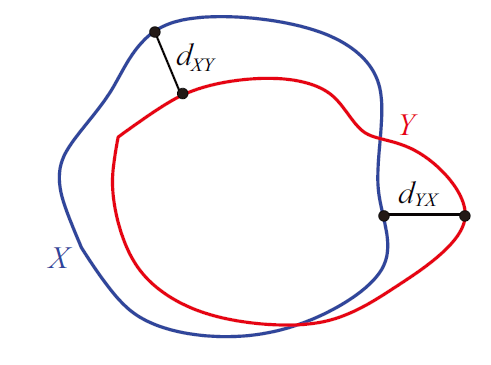
\includegraphics[width=0.4\linewidth]{imagenes/distanceHaussdorff.png}
		\caption{Distancias de Hausdorff entre dos conjuntos}
	\end{figure}
	
	Podemos enunciar la distancia máxima de Hausdorff:
	
	$$ H(A, B) = \max \left\{ \max_{a \in A} \min_{b \in B} d(a, b), \max_{b \in B} \min_{a \in A} d(a, b) \right\} $$
	
	Donde $a, b$ son puntos concretos en los conjuntos, $d(a, b)$ la distancia euclidiana entre los dos puntos y $A, B$ los conjuntos de puntos.
	
	Obtendremos la distancia de Hausdorff media de todos los slices de cada resonancia:
	
	$$ \bar{H}(A, B) = \frac{1}{|N|} \sum_{s \in N} H(A, B) $$
	
	De esta forma, a menor distancia de Hausdorff la segmentación salida y real son geométricamente más parecidas.
	
	\item \textbf{Sensibilidad o Recall} : Mide la proporción de casos positivos que fueron correctamente identificados por el modelo. En otras palabras y para nuestro problema, mide cuánto la segmentación predicción coincide con la segmentación verdadera, cuantificado en porcentaje.
	
	Podemos expresarlo como:
	
	$$ \text{Recall} = \frac{\text{TP}}{\text{TP} + \text{FN}} $$
	
	Donde $TP$ son los pixeles que son verdaderos positivos y $FN$ los pixeles que son falsos negativos.
	
\end{enumerate}

\section{Desarrollo para la predicción de la evolución}

Por falta de datos y recursos no pudimos entrar a resolver la predicción de la evolución de una lesión tumoral. Sin embargo, al menos teóricamente planteamos resolver esta tercera tarea. Es necesario tener en cuenta que la solución que aportaremos se sustenta en justo lo que no tuvimos, \textbf{más imágenes de una misma resonancia en diferentes momentos en el tiempo}. Se cree que la existencia de estos datos es una condición necesaria, ya que hasta el conocimiento que se tiene en este trabajo soluciones sin etiquetas no son viables.

Para construir una solución a este problema podemos valernos del \textbf{mismo encoder $g_{\phi}$ y representación latente $z$} utilizados en todas las arquitecturas con anterioridad. Posteriormente, podemos conectar un \textbf{Visual Transformer} que tenga como entrada la salida aplanada de la representación latente y tenga como output la segmentación en una instancia a corto plazo futura.

El objetivo del uso de una arquitectura transformadora es encontrar la correlación entre las \textbf{palabras} de entrada del decodificador (patches o píxeles de las imágenes) para poder minar \textbf{(si existen)} detalles en la imagen que lleven a poder predecir en el corto plazo cómo se extendería la lesión tumoral.

A continuación, podemos ver el esquema de este modelo hipótesis planteado.

\begin{figure}[H]
	\centering
	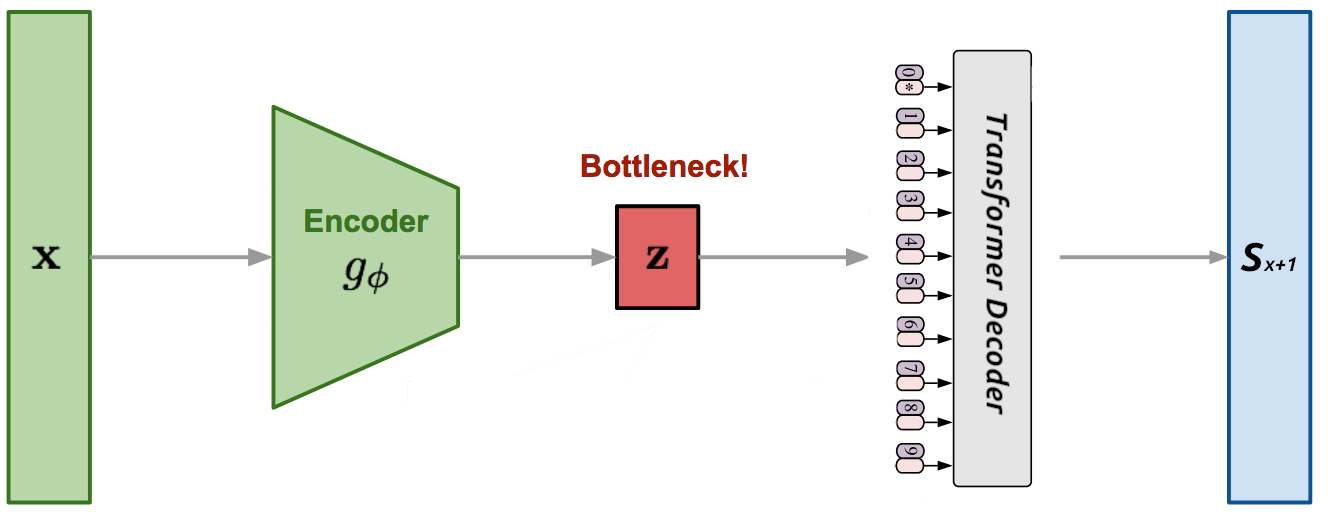
\includegraphics[width=0.9\linewidth]{imagenes/esquema_evolucion.png}
	\caption{Arquitectura propuesta para predicción de la evolución de los tumores}
\end{figure}

A continuación, hacemos algunas consideraciones de cómo llevar a cabo la optimización de esta arquitectura y detalles para poder llevarlo a la práctica.

\begin{enumerate}
	\item \textbf{Sigue siendo un problema de segmentación}. En la formulación del problema que estamos dando no estaríamos reconstruyendo la imagen futura sino su segmentación. Por lo tanto, pérdidas como \textbf{Dice Loss} seguirían siendo prometedoras.
	\item \textbf{Discretización del tiempo}. El tiempo es una magnitud que de forma precisa es discretizada en intervalos muy pequeños, por ejemplo podría ser discretizada en horas o minutos. En este problema carece de sentido una discretización demasiado precisa porque justamente lo interesante es ver las diferencias con la segmentación original para adelantarse a ellas. Un buen intervalo de discretización antes de entrenar el modelo y con datos en este intervalo son necesarios.
\end{enumerate}

\addcontentsline{toc}{chapter}{Experimentación}
\chapter{Experimentación}

En este capítulo se recoge el desarrollo de los experimentos llevados a cabo en este trabajo y todos los resultados que se han obtenido empíricamente de estos.

\section{Bibliotecas y desarrollo de los experimentos}

Para el desarrollo de los experimentos usaremos las bibliotecas de aprendizaje profundo \textbf{PyTorch} para la construcción de la estructura del proyecto y \textbf{Fastai} biblioteca extensión de PyTorch para el proceso de entrenamiento de los modelos. Construiremos nuestras propias clases en PyTorch para la construcción de las arquitectura y para la creación de la instancia de trabajo de nuestro dataset. Tenemos las siguientes componentes.

\begin{enumerate}
	\item \textbf{Clase del Dataset: BraTS}. Clase que representa al conjunto de datos. Sus funciones principales son \texttt{len(self)} que devuelve la cantidad de datos en la clase y \texttt{getitem(self, index)} que devuelve un dato de la clase dado un índice. Esta clase hereda de la clase \textbf{Dataset} de PyTorch.
	La instancia de esta clase será la entrada a la clase \textbf{DataLoader} de PyTorch.
	
	\item \textbf{Clases de las arquitecturas: SegNet y BinaryNet}. Implementan las arquitecturas para clasificación y segmentación. Aparte del constructor que es donde se define la arquitectura tiene la función \texttt{forward(self, x)} que define como se infiere por la red. PyTorch solo necesita la definición de la inferencia para calcular automáticamente la función \texttt{backward} internamente la función para la aplicación de backpropagation (necesario en el entrenamiento). Usa las instancias de los módulos siguientes.
	
	\item \textbf{Clases de los módulos de subida y bajada: DownConv y UpConv}. Análogas a las clases de la arquitecturas pero reduciéndolo a una parte. Usa la instancia de la clase siguiente (ya que sólo definimos uno de estos bloques por módulo).
	
	\item \textbf{Clase de un bloque de convolución: ConvBlock}. Clase que define las capas de un bloque de en nuestra red. Dentro del constructor llama a las funciones de PyTorch de ReLU, convolución y batch normalization.
	
\end{enumerate}

A continuación, podemos ver en detalle la estructura de todos nuestros experimentos a través de un diagrama de clases.

\begin{figure}[H]
	\centering
	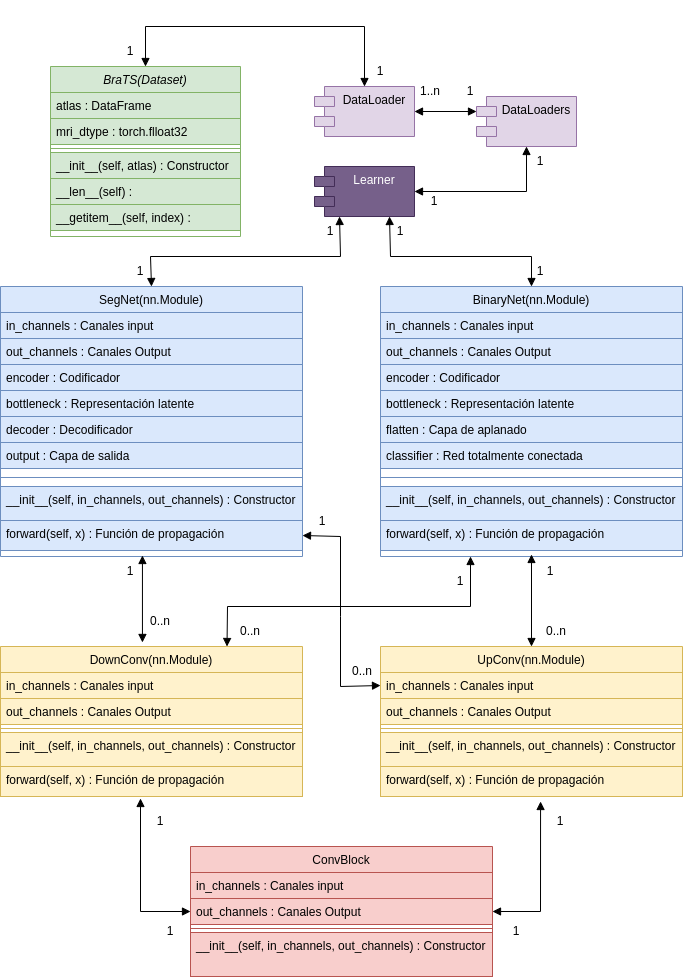
\includegraphics[width=0.75\linewidth]{imagenes/clases_pytorch.png}
	\caption{Diagrama de clases de PyTorch}
\end{figure}

\section{Construcción del codificador y representación latente}

Pasamos a comentar los experimentos llevados cabo en la tarea de la reconstrucción de imágenes.

\subsection{Arquitecturas con conexiones residuales: ResNet34}

Comenzamos ajustando \textbf{ResNet34} a las imágenes. Tras $7$ épocas sumando un total de $8$ horas $30$ minutos de entrenamiento para toda la red obtenemos estos resultados.
Podemos ver los resultados en forma tabular y en forma de gráfica. En la gráfica el eje $Y$ representa la pérdida y el eje $X$ representa la cantidad de imágenes vistas (aunque haya visto la misma imagen más de una vez en distintas épocas). 

\begin{table}[H]
	\centering
	\begin{tabular}{|ccccc|}
		\toprule
		epoch & train\_loss & valid\_loss & MAE & time \\ 
		\midrule
		0 & 0.098790 & 0.111301 & 0.111301 & 1:09:46 \\ 
		0 & 0.079261 & 0.081548 & 0.081548 & 1:13:33 \\
		2 & 0.071293 & 0.075421 & 0.075421 & 1:14:20 \\ 
		3 & 0.064748 & 0.067580 & 0.067580 & 1:14:41 \\ 
		4 & 0.059911 & 0.062933 & 0.062933 & 1:15:55 \\ 
		5 & 0.057501 & 0.059307 & 0.059307 & 1:15:36 \\ 
		6 & 0.055986 & 0.058405 & 0.058405 & 1:15:37 \\ 
		\bottomrule
	\end{tabular}
	\caption{Pérdida de entrenamiento y validación para la reconstrucción con ResNet34}
	\label{tabla:resultados2}
\end{table}

\begin{figure}[H]
	\centering
	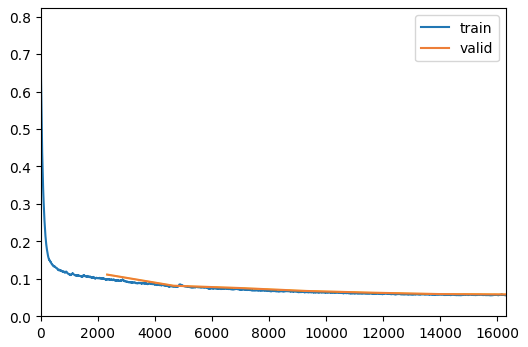
\includegraphics[width=0.7\linewidth]{imagenes/curva_resnet34.png}
	\caption{Curva de aprendizaje con ResNet34}
\end{figure}

Observamos una rápida convergencia la inicio y un entrenamiento perfecto con ambos errores muy cercanos en todas las épocas $E_{val} \approx E_{train}$. Indicando que el proceso de entrenamiento está realizando correctamente y que la arquitectura es válida para aprender a reconstruir las imágenes. Finalmente, obtenemos un $E_{val} \approx 0.058$ lo cual indica que nuestra red reconstruye las imágenes con una pérdida del $5.8 \%$ de los detalles reales.

A continuación, observamos cómo la red reconstruye tres imágenes. En la siguiente salida vemos tres imágenes donde podemos apreciar la salida de la red como la imagen de la izquierda de cada pareja y la imagen real a la derecha.

\begin{figure}[H]
	\centering
	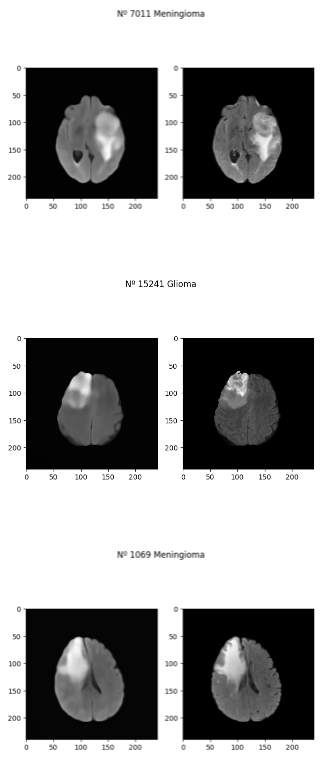
\includegraphics[width=0.4\linewidth]{imagenes/reconstruccion_resnet34.png}
	\caption{Reconstrucción de las imágenes con ResNet34}
\end{figure}

\subsection{Arquitecturas con filtros con distinto tamaño: Xception}

Dentro de las pruebas para elegir el mejor codificador seguimos con la prueba de bondad de \textbf{Xception}. Lo evaluamos en las mismas condiciones que \textbf{ResNet34}.

\begin{table}[H]
	\centering
	\begin{tabular}{|ccccc|}
		\toprule
		epoch & train\_loss & valid\_loss & MAE & time \\ 
		\midrule
		0 & 0.102650 & 0.105854 & 0.105854 & 1:24:38 \\ 
		1 & 0.083989 & 0.089979 & 0.089979 & 1:28:34 \\ 
		2 & 0.074420 & 0.085525 & 0.085525 & 1:28:33 \\ 
		3 & 0.068684 & 0.071334 & 0.071334 & 1:30:09 \\ 
		4 & 0.063998 & 0.065802 & 0.065802 & 1:26:00 \\ 
		5 & 0.060919 & 0.063771 & 0.063771 & 1:27:03 \\ 
		6 & 0.060293 & 0.062978 & 0.062978 & 1:26:51 \\ 
		\bottomrule
	\end{tabular}
	\caption{Pérdida de entrenamiento y validación para la reconstrucción de Xception}
	\label{tabla:resultados}
\end{table}

\begin{figure}[H]
	\centering
	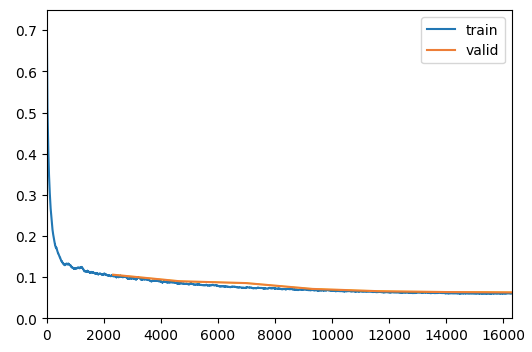
\includegraphics[width=0.7\linewidth]{imagenes/curva_xception.png}
	\caption{Curva de aprendizaje con Xception}
\end{figure}

Observamos una más rápida convergencia que \textbf{ResNet34} motivado posiblemente por los filtros de distintos tamaños. Tenemos el mismo comportamiento de bondad entre la pérdida de entrenamiento y validación. Sin embargo, obtenemos una pérdida en validación de $E_{val} \approx 0.062$ la cual es superior a la de \textbf{ResNet34} indicando que a pesar de la rápida convergencia el resultado final es mejor con un mayor número de conexiones residuales. 

A continuación observamos su reconstrucción con un resultado muy similar en apariencia.
\begin{figure}[H]
	\centering
	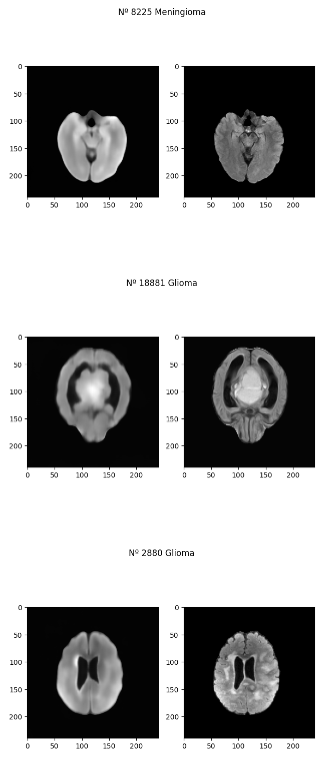
\includegraphics[width=0.4\linewidth]{imagenes/reconstruccion_xception.png}
	\caption{Reconstrucción de las imágenes con Xception}
\end{figure}

A continuación, ante los resultados de esta comparación mostramos la siguiente tabla.

\begin{table}[H]
	\centering
	\begin{tabular}{|cccccc|}
		\toprule
		Arquitectura & $E_{train}$ & $E_{val}$ \\ 
		\midrule
		\textbf{ResNet34} & \textbf{0.055986} & \textbf{0.058405} \\ 
		Xception & 0.060293 & 0.062978 \\ 
		\bottomrule
	\end{tabular}
	\caption{Pérdida de entrenamiento y validación para clasificación con la parte convolucional congelada}
	\label{tabla:resultados3}
\end{table}

Eligiendo por tanto a \textbf{ResNet34} como codificador de las arquitecturas. 

\section{Clasificación}

\subsection{Entrenamiento en clasificación}

A continuación, mostramos los experimentos realizados para la tarea de clasificación. Tomamos \textbf{ResNet34} como codificador le añadimos la representación latente y las capas densamente conectadas, entrenamos las capas fully-connected congelando las capas convolucionales (codificador y representación latente) durante $3$ épocas tomando $\approx 3$ horas con estos resultados.

\begin{table}[H]
	\centering
	\begin{tabular}{|cccccc|}
		\toprule
		epoch & train\_loss & valid\_loss & accuracy & balanced\_accuracy & time \\ 
		\midrule
		0 & 0.112794 & 0.178968 & 0.805254 & 0.781898 & 1:04:50 \\ 
		1 & 0.119699 & 0.174729 & 0.819330 & 0.773066 & 1:03:01 \\ 
		\textbf{2} & \textbf{0.083459} & \textbf{0.141255} & \textbf{0.855540} & \textbf{0.794527} & \textbf{1:04:18} \\ 
		\bottomrule
	\end{tabular}
	\caption{Pérdida de entrenamiento y validación para clasificación con la parte convolucional congelada}
	\label{tabla:resultados3}
\end{table}

\begin{figure}[H]
	\centering
	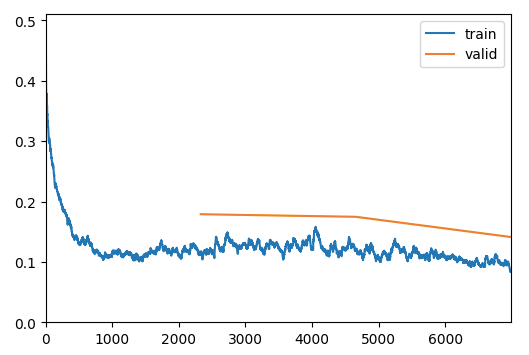
\includegraphics[width=0.7\linewidth]{imagenes/task1_freeze.png}
	\caption{Curva de aprendizaje para clasificación parte convolucional congelada}
\end{figure}

Observamos una rápida convergencia al inicio del entrenamiento, estabilizándose durante la época número $1$ y volviendo a converger ligeramente durante la época $2$. En este caso y para esta primera fase, el entrenamiento no es tan óptimo, habiendo cierta distancia entre las pérdidas de validación y entrenamiento. 

A continuación, tras estas $3$ épocas ajustando las capas densamente conectadas pasamos a descongelar toda la red para que quede mejor ajustado.

\begin{table}[H]
	\centering
	\begin{tabular}{|cccccc|}
		\toprule
		epoch & train\_loss & valid\_loss & accuracy & balanced\_accuracy & time \\
		\midrule
		0 & 0.056434 & 0.209338 & 0.855477 & 0.840139 & 1:01:57 \\ 
		\textbf{1} & \textbf{0.040761} & \textbf{0.190361} & \textbf{0.864976} & \textbf{0.812309} & \textbf{1:01:41} \\ 
		2 & 0.023256 & 0.260177 & 0.876575 & 0.832247 & 1:00:26 \\ 
		3 & 0.009723 & 0.330192 & 0.877014 & 0.834721 & 1:00:30 \\ 
		\bottomrule
	\end{tabular}
	\caption{Pérdida de entrenamiento y validación para clasificación toda la red descongelada}
	\label{tabla:resultados3}
\end{table}

\begin{figure}[H]
	\centering
	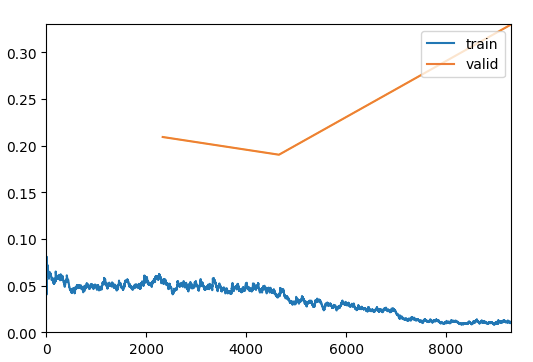
\includegraphics[width=0.7\linewidth]{imagenes/task1_unfreeze.png}
	\caption{Curva de aprendizaje para clasificación toda la red descongelada tras ajustar capas densamente conectadas}
\end{figure}

Observamos como en las dos primeras épocas tenemos convergencia en validación, tras ellos se dispara validación indicándonos que hemos llegado al resultado tope en el entrenamiento. Este proceso de entrenamiento esta configurado con \textbf{EarlyStopping} por lo que PyTorch automáticamente guarda el mejor modelo (el que haya conseguido una pérdida en validación más baja en todas las épocas) en este caso tras descongelar obtiene como modelo final el correspondiente a la época número $1$. 

Observamos como tras haber pasado el proceso de ajuste inicial de las capas densamente conectadas al descongelar todo, obtenemos unas pérdida de validación y entrenamiento mucho más dispares. Esto podría cómo las diferentes partes de la arquitectura inducen complejidad en el proceso de entrenamiento: las capas densamente conectadas (que era lo único entrenable en la primera fase) hacen que esta diferencia sea muy pequeña porque estas capas son en comparación pequeñas. Al descongelar toda las capas de la red, siendo el codificador mucho mayor que las capas densas se observa como se induce un ruido mayor.


A continuación, y a pesar de que la teoría indica que primero ajustemos las capas densamente conectadas primero congelando el resto de las capas en sus inicios, probamos a entrenar toda la red descongelada sin un ajuste previo.

\begin{table}[H]
	\centering
	\begin{tabular}{|cccccc|}
		\toprule
		epoch & train\_loss & valid\_loss & accuracy & balanced\_accuracy & time \\
		\midrule
		0 & 0.080457 & 0.178836 & 0.854348 & 0.796523 & 1:23:49 \\ 
		1 & 0.084583 & 0.175143 & 0.847827 & 0.781100 & 1:24:09 \\ 
		\textbf{2} & \textbf{0.086810} & \textbf{0.159217} & \textbf{0.852185} & \textbf{0.800501} & \textbf{1:26:20} \\ 
		3 & 0.081304 & 0.370888 & 0.832309 & 0.747997 & 1:21:31 \\ 
		\bottomrule
	\end{tabular}
	\caption{Pérdida de entrenamiento y validación para clasificación para todo el entrenamiento toda la red descongelada}
	\label{tabla:resultados6}
\end{table}


\begin{figure}[H]
	\centering
	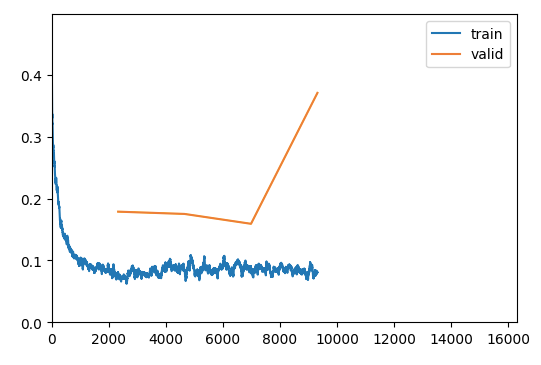
\includegraphics[width=0.7\linewidth]{imagenes/task1_totally_unfreeze.png}
	\caption{Curva de aprendizaje para clasificación todo el entrenamiento toda la red descongelada}
\end{figure}

Observamos como el mejor resultado que obtenemos es en la época número $2$ siendo peor que la mejor con la estrategia anterior. Adicionalmente, observamos como se alcanza una convergencia rápida llevando a fuerte overfitting justo en la siguiente época. Podemos interpretar como esta estrategia no sólo da peores resultados sino tiene una peor estabilidad en el proceso de entrenamiento.

\subsection{Validación en clasificación}

Tras entrenar los modelos pasamos a obtener los resultados finales infiriendo con el modelo en clasificación para los conjuntos de validación y test.

\subsubsection{Antes de aplicar votación}

En primer lugar calculamos la bondad sin aplicar el esquema de votación, la esperanza que se tiene es que tras la aplicación el esquema de votación los resultados sean iguales o mejores que los siguiente. No aplicaremos test ya que la tarea real es clasificación binaria con el esquema por lo que no es relevante el resultado de test en estas condiciones. 

A continuación, vemos los resultados obtenidos de ajuste para las métricas en entrenamiento y validación sin votación. Construimos las siguientes matrices de confusión tras la inferencia de cada conjunto.
 
\begin{figure}[H]
	\centering
	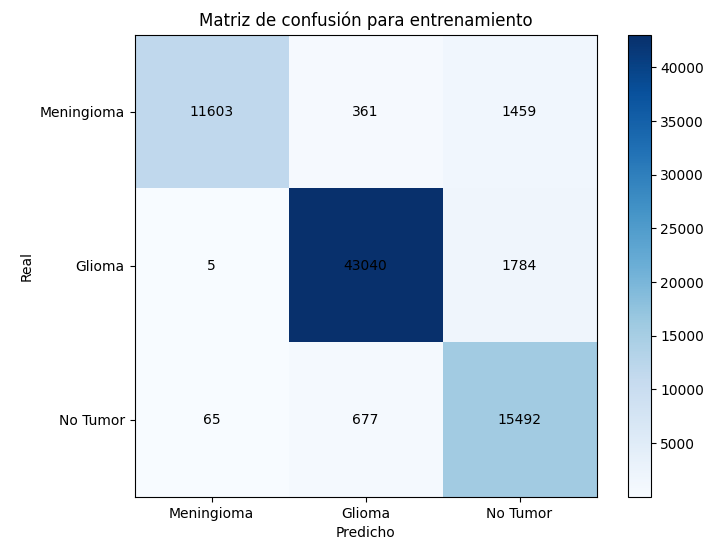
\includegraphics[width=0.7\linewidth]{imagenes/task1_results_train.png}
	\caption{Matriz de confusión de entrenamiento sin votación}
\end{figure}

\begin{figure}[H]
	\centering
	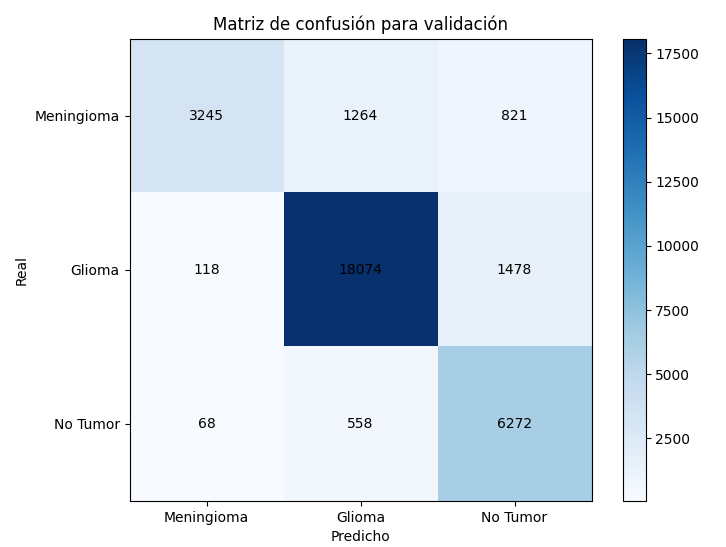
\includegraphics[width=0.7\linewidth]{imagenes/task1_results_validation.png}
	\caption{Matriz de confusión de validación sin votación}
\end{figure}

\begin{table}[H]
	\centering
	\begin{tabular}{|ccc|}
		\toprule
		Conjunto & accuracy ($\%$) & balanced\_accuracy ($\%$) \\
		\midrule
		Entrenamiento & 94.1586 & 92.6266 \\ 
		Validación & 86.4976 & 81.2309 \\ 
		\bottomrule
	\end{tabular}
	\caption{Resultados de validación y entrenamiento sin votación}
	\label{tabla:resultados10}
\end{table}

Observamos un ajuste alto en los datos de entrenamiento indicando un buen proceso de entrenamiento y resultados competitivos pero mejorables en validación. Observamos como la clase más conflictiva es \textbf{No Tumor} con las otras dos clases de tumores, indicando que la tarea más difícil es la detección del tumor y no la caracterización de este.

\subsubsection{Tras aplicar votación}

Aplicamos el esquema de votación, en primer lugar necesitamos explorar el parámetro $threshold$ que definimos en la metodología. El parámetro $threshold$ mide la tolerancia que tiene el modelo para predecir a meningioma, cuando existe un mayor número de predicciones por imagen a meningioma que $threshold$ el modelo predice toda la resonancia a meningioma, y en caso contrario a glioblastoma.

Tras hacer inferencia y ver qué cantidad promedio de predicciones de cada clase obteníamos para toda la resonancia de unos cuantos ejemplos, observamos como las predicciones a meningiomas eran muchos menores que para los gliomas. Esto está motivado por la propia naturaleza de la cantidad de imágenes de tumores de cada clase debido a que los meningiomas son más pequeños que los gliomas en promedio. 

Como definimos en la metodología necesitamos un esquema que lidie con este desbalanceo. Por ello, descartamos valores altos de $threshold$ y probamos dos valores pequeños: para $threhold = 5$ y $threshold = 3$.

A continuación mostramos las matrices de confusión asociadas a la aplicación de estos dos esquemas de votación.

\begin{figure}[H]
	\centering
	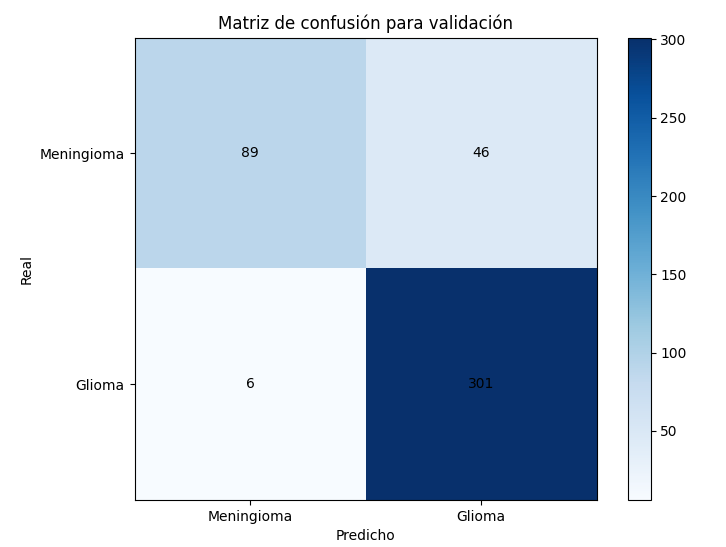
\includegraphics[width=0.7\linewidth]{imagenes/task1_val_5.png}
	\caption{Matriz de confusión de validación con votación: $Meningiomas < 5$}
\end{figure}

\begin{figure}[H]
	\centering
	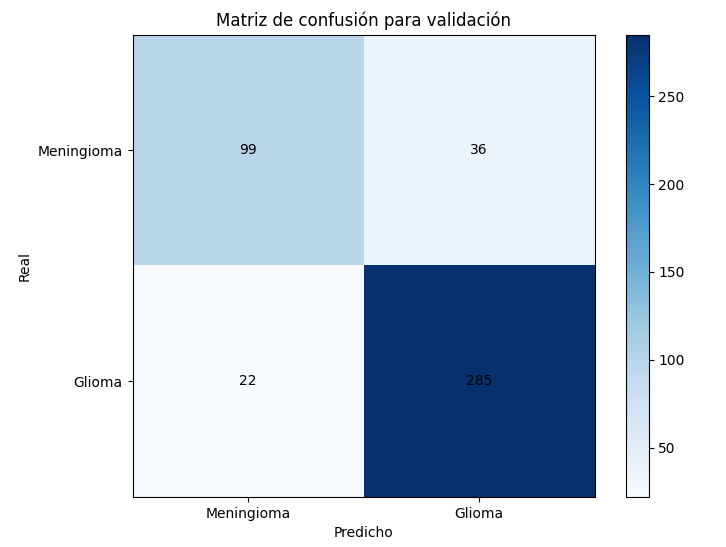
\includegraphics[width=0.7\linewidth]{imagenes/task1_val_3.png}
	\caption{Matriz de confusión de validación con votación: $Meningiomas < 3$}
\end{figure}

\begin{table}[H]
	\centering
	\begin{tabular}{|ccc|}
		\toprule
		Threshold & accuracy ($\%$) & balanced\_accuracy ($\%$) \\
		\midrule
		5 & 88.2352 & 81.9857 \\ 
		3 & 86.8779 & 83.0363  \\ 
		\bottomrule
	\end{tabular}
	\caption{Resultados de validación con votación y de la búsqueda}
	\label{tabla:resultados11}
\end{table}

Observamos como obtenemos un mejor accuracy balanceado con $threshold = 3$, así que optamos por su elección.
Tras haber configurado $threshold = 3$ y haber visto su bondad en validación solo queda obtener el resultado final con test.

\begin{figure}[H]
	\centering
	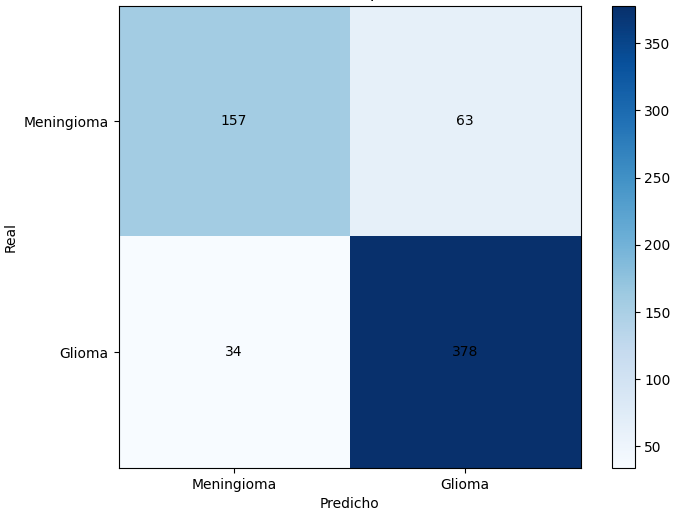
\includegraphics[width=0.8\linewidth]{imagenes/task1_test.png}
	\caption{Matriz de confusión de Test con votación}
\end{figure}

Obtenemos resultados finales para test, obteniendo un accuracy del $84.6519 \%$ y un accuracy balanceado del $81.5556 \%$. Con este resultado sabemos que la obtención de un modelo final debería tener un accuracy balanceado en clasificación $ Acc_{F} \geq 81.5556 \% $.

\subsection{Comparativa de clasificación con el estado del arte}

Para finalizar la experimentación de esta primera tarea ponemos en contexto estos resultados con el estado del arte. Aunque no sean del todo comparables debido no son formulaciones del problema idénticas (se tiene otro tipo de tumor en el estado del arte) y se utilizan conjuntos de datos distintos T1-CE image en el estado del arte frente a BraTS en el este trabajo. Sin embargo, es importante hacer una observación de la bondad de los resultados teniendo en cuenta estas diferencias. 

\begin{table}[H]
	\centering
	\begin{tabular}{|cccc|}
		\toprule
		Autor & accuracy ($\%$) & balanced\_accuracy ($\%$) & $P_{test}$ \\
		\midrule
		\cite{cheng2015enhanced} & 91.2 & - & 61\\ 
		\cite{cheng2016retrieval} & 94.7 & - & 61\\ 
		\cite{abiwinanda2019brain} & 84.1 & - & 70\\ 
		\cite{pashaei2018brain} & 81.0 & - & 70\\ 
		\cite{sultan2019multi} & 96.1 & - & 75\\
		\cite{diaz2021deep} & 97.3 & - & 46 \\  
		Nuestro método & 84.65 & 81.56 & 632 \\ 
		\bottomrule
	\end{tabular}
	\caption{Resultados de validación con votación y de la búsqueda}
	\label{tabla:resultados12}
\end{table}

Los resultados del estado del arte no incluyen un validación con un esquema balanceado lo cual lo hace soluciones mucho menos generales y reales. Añadimos a la tabla, la entrada $P_{test}$ que la cantidad de pacientes que se usaron en el conjunto de test de cada trabajo.

Nuestro trabajo está validado en un conjunto de test $\approx 8$ veces mayor que el mayor conjunto utilizado en la literatura y utiliza una política de aprendizaje balanceado lo cual puede hacer obtener peores resultados en un métrica más débil como puede ser accuracy sin balanceo. Aún así nuestro método supera a 2 de los 6 métodos presentados en la revisión histórica.

\section{Segmentación}

En esta sección recogemos los experimentos y resultados de estos para la tarea de segmentación. 

\subsection{Entrenamiento en segmentación}
Entrenamos la arquitectura enteramente descongelada con tamaño de lote de $32$ ejemplos durante $7$ épocas alcanzando el entrenamiento una duración de $ \approx 8$ horas. A continuación se presenta la tabla y curva de aprendizaje obtenidas.
\begin{table}[H]
	\centering
	\begin{tabular}{|ccccc|}
		\toprule
		epoch & train\_loss & valid\_loss & Dice Loss & time \\ 
		\midrule
		0 & 0.095941 & 0.319656 & 0.319656 & 1:34:08 \\ 
		\textbf{1} & \textbf{0.073242} & \textbf{0.258797} & \textbf{0.258797} & \textbf{1:32:56} \\ 
		2 & 0.059904 & 0.284256 & 0.284256 & 1:34:48 \\ 
		3 & 0.050076 & 0.274452 & 0.274452 & 1:37:00 \\ 
		4 & 0.046783 & 0.266702 & 0.266702 & 1:40:18 \\ 
		\bottomrule
	\end{tabular}
	\caption{Pérdida de entrenamiento y validación para segmentación toda la red descongelada}
	\label{tabla:resultados4}
\end{table}

\begin{figure}[H]
	\centering
	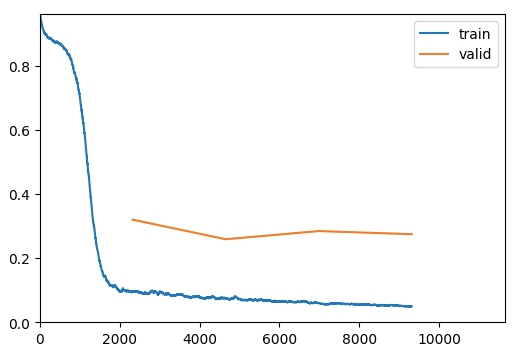
\includegraphics[width=0.7\linewidth]{imagenes/curva_segmentation.png}
	\caption{Curva de aprendizaje para la tarea de segmentación}
\end{figure}

Observamos como tenemos una muy rápida convergencia en la primera época y cómo se estabiliza en las sucesivas épocas refinándose la pérdida Dice muy ligeramente. En este tiempo de cómputo limitado observamos como no se produce overfitting. Sin embargo, obtenemos un error de validación que disminuye muy poco entre la primera y segunda época aumentando ligeramente en las sucesivas épocas. Podemos interpretar que existe un comportamiento estable en todo el proceso de entrenamiento.

A continuación, comparamos la salida del modelo respecto la imagen real. Esta salida es previa a aplicarle un proceso de umbralización con la cual obtendríamos una máscara binaria final. El proceso de umbralización que se aplicará consiste en determinar como píxeles segmentados (usando la etiqueta 1) los píxeles cuyo valor sea mayor a un umbral $U$ y en caso contrario, píxeles no segmentados (usando la etiqueta 0). El umbral $U$ empleado será $U = 0.8$. Viendo en la práctica como este umbral o uno ligeramente más bajo como $0.5$ no afecta significativamente a los resultados. 
\begin{figure}[H]
	\centering
	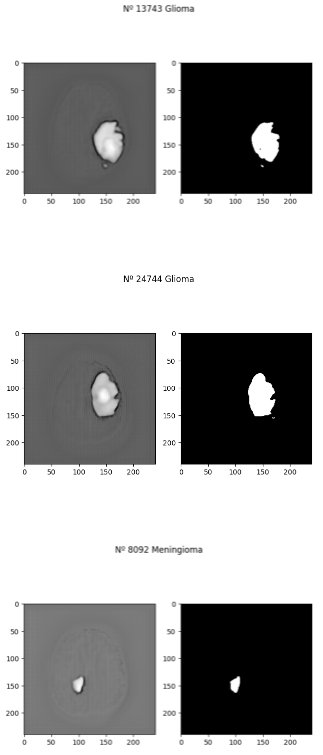
\includegraphics[width=0.5\linewidth]{imagenes/output_segmentation.png}
	\caption{Comparación de la salida del modelo respecto la real}
\end{figure}
Observamos buenos resultados consiguiendo máscaras de segmentación que replican en detalle la segmentación original. En la imagen producida por la red se puede apreciar la sombra de un cerebro pudiendo ver un efecto residual del codificador y del uso de skip connections.

\subsection{Validación en segmentación}

A continuación, inferimos los resultados finales para segmentación en validación y test para nuestras tres métricas. Recogemos en la siguiente tabla estos resultados.

\begin{table}[H]
	\centering
	\begin{tabular}{|cccc|}
		\toprule
		Partición & Similaridad Dice & Distancia Hausdorff & Sensibilidad \\ 
		\midrule
		Validación & 0.777343 & 14.573561 & 0.720415 \\ 
		Test & 0.772642 & 14.577154 & 0.709075 \\ 
		\bottomrule
	\end{tabular}
	\caption{Resultados de hold-out en validación y test para segmentación}
	\label{tabla:resultados5}
\end{table}
Observamos que ambos conjuntos mantienen resultados muy similares empeorando ligeramente en test indicando robustez y coherencia en los resultados. Observamos que la peor métrica obtenida es la distancia Hausdorff que es demasiado alta, indicando que existe una distancia máxima media de $\approx 14$ píxeles entre la segmentación original y la salida del modelo. Podría significar un problema de creación de artefactos por parte del modelo.

A continuación, para darle explicabilidad a los resultados se muestra el histograma de los resultados de las métricas para todos los ejemplos, primero del conjunto de validación y después para el conjunto de test. De esta forma, podríamos identificar ejemplos especialmente difíciles y caracterizarlos.
\begin{figure}[H]
	\centering
	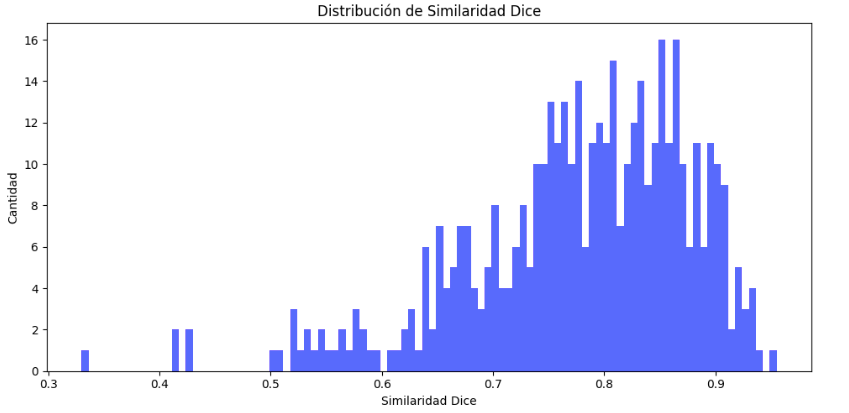
\includegraphics[width=0.7\linewidth]{imagenes/dist_dice_val.png}
	\caption{Distribución de similaridad Dice en el conjunto de validación}
\end{figure}

\begin{figure}[H]
	\centering
	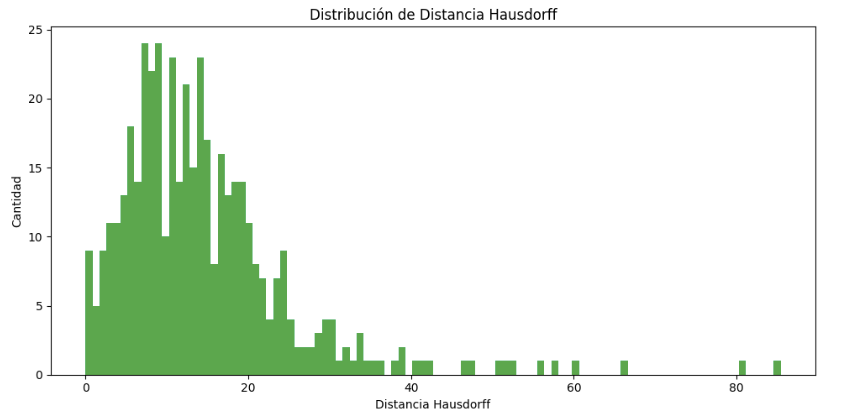
\includegraphics[width=0.7\linewidth]{imagenes/dist_haus_val.png}
	\caption{Distribución de distancia Hausdorff en el conjunto de validación}
\end{figure}

\begin{figure}[H]
	\centering
	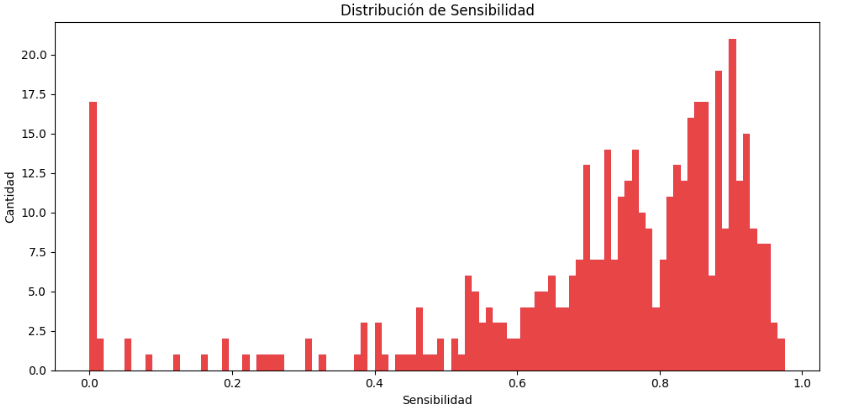
\includegraphics[width=0.7\linewidth]{imagenes/dist_sen_val.png}
	\caption{Distribución de sensibilidad en el conjunto de validación}
\end{figure}

\begin{figure}[H]
	\centering
	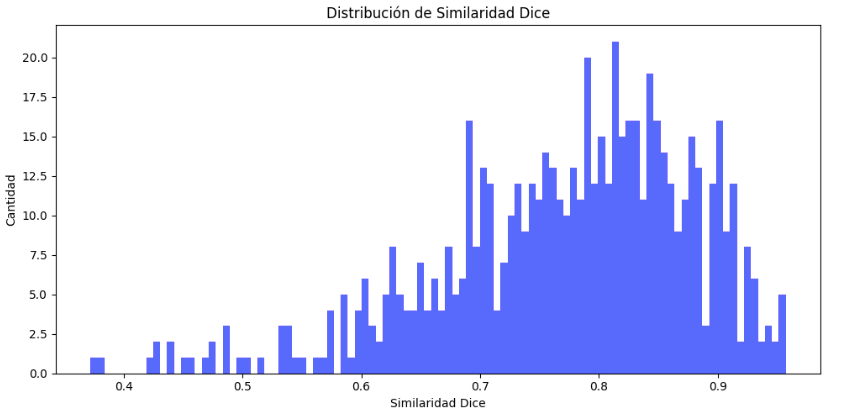
\includegraphics[width=0.7\linewidth]{imagenes/dist_dice_test.png}
	\caption{Distribución de similaridad Dice en el conjunto de test}
\end{figure}

\begin{figure}[H]
	\centering
	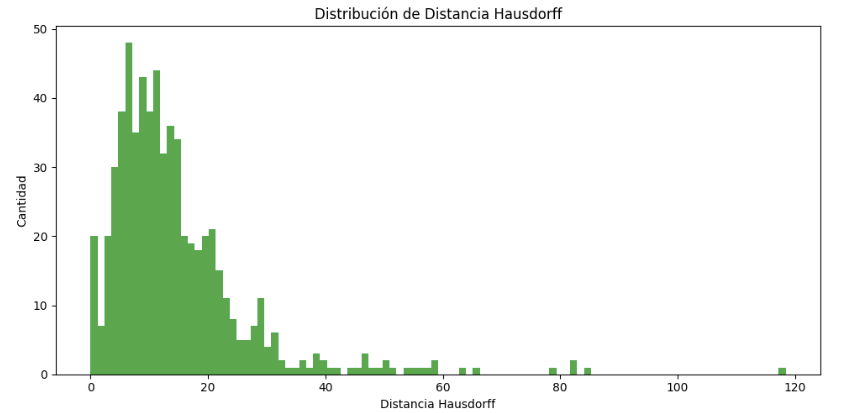
\includegraphics[width=0.7\linewidth]{imagenes/dist_haus_test.png}
	\caption{Distribución de distancia Hausdorff en el conjunto de test}
\end{figure}

\begin{figure}[H]
	\centering
	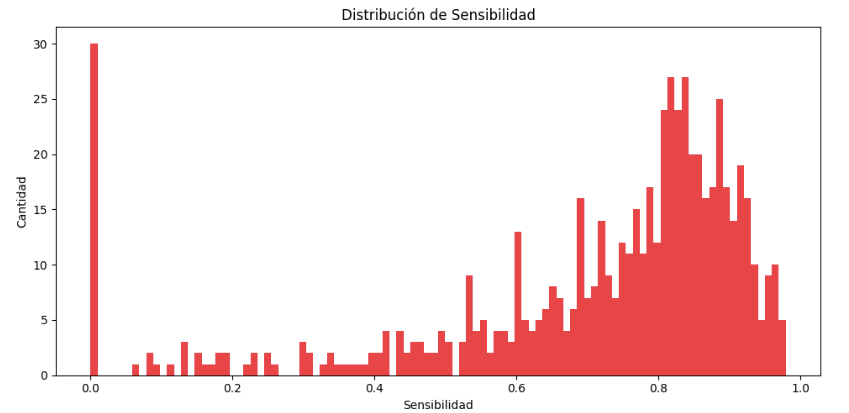
\includegraphics[width=0.7\linewidth]{imagenes/dist_sen_test.png}
	\caption{Distribución de sensibilidad en el conjunto de test}
\end{figure}

Los histogramas de estas métricas revelan una distribución en forma de campana de Gauss, lo cual es indicativo de una distribución normal. Este patrón indica robustez dentro del modelo de segmentación, observando que no existe un subconjunto de ejemplos que no puede segmentar bien. Nos sirve como prueba para demostrar la generalidad del modelo conseguida a pesar de poder obtener un modelo mejor.

La normalidad de las distribuciones también implica que las métricas son simétricas y centradas alrededor de un valor promedio consistente, lo que es indicativo de un rendimiento estable.

\subsection{Comparativa de segmentación con el estado del arte}

Para finalizar la experimentación de esta segunda tarea ponemos en contexto estos resultados con el estado del arte. Todos estos resultados han sido evaluados por conjuntos de mismo dataset \textbf{BraTS}, y respetando la misma proporción entre entrenamiento-test que la seguida en este trabajo.

En la siguiente tabla se muestran las métricas y un apartado de recursos que indica la GPU que usaron para el entrenamiento. En nuestro método usamos una gráfica Tesla P100 limitados semanalmente $30$ horas y en cada ejecución a $12$ horas. Por lo que, no podemos entrenar más de $12$ horas seguidas.

\begin{table}[H]
	\centering
	\begin{tabular}{|ccccc|}
		\toprule
		Autor & Dice ($\%$) & Hausdorff & Recall ($\%$) & Recursos \\
		\midrule
		\cite{chen2021transunet} & 78.73 & 5.0 & - & 8 x Tesla V100 \\
		\cite{zhou2021latent} & 87.1 & 6.5 & 86.8 & Quadro P5000 \\
		\cite{myronenko20193d} & 90.4 & 4.4 & - & 8 x Tesla V100\\   
		\cite{hatamizadeh2021swin} & 92.6 & 5.8 & - & 8 x Tesla V100 \\ 
		\cite{ferreira2024we} & 92.9 & 4.26 & - & 6 x RTX 6000\\
		Nuestro método & 77.3 & 14.5 & 70.9 & Tesla P100 \\ 
		\bottomrule
	\end{tabular}
	\caption{Comparativa de segmentación con el estado del arte}
	\label{tabla:resultados13}
\end{table}

Como vemos nuestro método es peor que todo el estado del arte reciente que sea comparable. Sin embargo, es una buena aproximación para las capacidades de recursos en términos de capacidad (memoria del dispositivo GPU) y rendimiento de GPU que teníamos frente las del resto de autores que son inmensamente mayores. 


%\chapter{Conclusiones y Trabajos Futuros}
%
%
%\nocite{*}
\bibliographystyle{plain}
\bibliography{bibliografia/bibliografia}\addcontentsline{toc}{chapter}{Bibliografía}

%
%\appendix
%\input{apendices/manual_usuario/manual_usuario}
%%\input{apendices/paper/paper}
%\newglossaryentry{prevalencia}{
    name=prevalencia,
    description={En epidemiología, proporción de personas que sufren una enfermedad con respecto al total de la población en estudio}
}
\newglossaryentry{maths}{
    name=mathematics,
    description={Mathematics is what mathematicians do}
}

% \addcontentsline{toc}{chapter}{Glosario}
% \printglossary
\chapter*{}
\thispagestyle{empty}

\end{document}
